\chapter{Проверка выдвинутых положений и рекомендации разработчикам}

В данной главе описаны эксперименты,
проведённые для подтверждения утверждений из~предыдущих глав. Описаны
исследования и практический опыт по снижению остаточных напряжений
посредством термообработки. Предложена методика минимизации остаточных
напряжений, представленная в виде шагов для разработчика прибора.
Также описаны сложности, на которые стоит обратить внимание при
разработке современной электронной техники с применением технологии
электростатического соединения.

\section{Определение остаточных напряжений в стекле}
\subsection{Описание метода поляризационно-оптического измерения разности хода лучей}\label{chap:measure_glass_stress}
<<Метод основан на явлении двулучепреломления, которое наблюдается в~напряжённом стекле при прохождении через него луча линейно-поляризованного света, и заключается в разложении луча на два: обыкновенный и~необыкновенный, распространяющиеся с различными скоростями и~вследствие этого имеющие при выходе из напряжённого
стекла разность хода>>~\cite{gost_metod_opred_dvulucheprelom}.

<<Метод включает качественное, полуколичественное и количественное определение
напряжения, исходя из разности хода поляризованного света, проходящего через
образец>>~\cite{gost_metod_opred_dvulucheprelom}.
При качественном и полуколичественном определении <<испытание проводят
способом сравнения, который состоит в~оценке на~полярископе общего
распределения напряжений в~изделии и~в~оценке значения разности
хода>>~\cite{gost_metod_opred_dvulucheprelom} сравнением наблюдаемого цвета одним из~двух способов:
\begin{itemize}
    \item <<с данными
    таблицы интерференционных цветов>>~\cite{gost_metod_opred_dvulucheprelom};
    \item <<с соответствующим цветом
    правильно ориентированного ступенчатого клина, или же одинакового
    изделия с количественно оценёнными разностями хода на обозначенных
    местах>>~\cite{gost_metod_opred_dvulucheprelom}.
\end{itemize}

При количественном определении напряжений <<испытание проводят способом
компенсации, который состоит в количественном определении значения разности хода
с помощью поляриметра, снабжённого компенсатором. В качестве компенсатора
применяют четвертьволновую фазовую пластинку с поворотным анализатором (компенсатор
Сенармона)>>~\cite{gost_metod_opred_dvulucheprelom}.
Четвертьволновая фазовая пластинка (фазовая пластинка $\lambda/$4) "---
<<устройство, создающее разность фаз между ортогональными линейно-поляризованными
составляющими оптического излучения определенной длины волны, равную
\((2n+1)\frac{\pi}{2}\), что соответствует разности хода между этими
составляющими, равной \((2n+1)\frac{\lambda}{4}\),
где \( n \) "--- целое число>>~\cite{gost_metod_opred_dvulucheprelom},
\( \lambda \) "--- длина волны света, нм.

<<При измерении разности хода с помощью поляриметра лимб анализатора устанавливают
на нулевую отметку, вводят пластину $\lambda/$4 и зелёный светофильтр.
Анализатор поворачивают на несколько градусов в обе стороны и для компенсации
выбирают то направление поворота анализатора, при котором тёмные полосы
приближаются к месту измерения. Медленно вращают анализатор до тех пор, пока
наблюдаемые в поле зрения тёмные полосы не сольются в одну утолщённую. Затем
анализатор слегка поворачивают в~обратную сторону, в~результате чего образуется
небольшой просвет между полосами, которые затем снова доводят до
соприкосновения. Угол поворота анализатора определяют по~лимбу анализатора. Для
расчёта разности хода применяют среднее значение результатов трёх
отсчётов>>~\cite{gost_metod_opred_dvulucheprelom}.

<<Разность хода ($\Delta$) в нанометрах вычисляют по формуле:
\begin{equation*}
    \Delta =\frac{\lambda \phi }{180}=3\phi,
\end{equation*}
где $\lambda$ "--- длина волны света, равная 540~нм при условии применения зелёного светофильтра;
$\phi$ "--- угол поворота анализатора>>~\cite{gost_metod_opred_dvulucheprelom}.

<<Удельную разность хода ($\Delta'$) в
10\textsuperscript{$-$6}
вычисляют по формуле:
\begin{equation*}
    \Delta'=\frac{\Delta}{l},
\end{equation*}
где $\Delta $ "--- разность хода, нм;
$ l $ "--- длина пути луча в напряжённом стекле, нм>>~\cite{gost_metod_opred_dvulucheprelom}.

\subsection{Результаты и обсуждение}
Были проведены эксперименты по соединению пластин кремния и стекла.
Использовались пластины кремния марки КЭС (кремний электронного типа проводимости, легирующий элемент "--- сурьма)
диаметром 60 мм ориентации \{100\} с~удельным сопротивлением 0,01 Ом$\cdot$см и прямоугольные пластины стекла ЛК5
размерами 30\(\,\times\,\)50\(\,\times\,\)4,5~мм. Соединения были проведены при
температуре от~330 до~350~{\textdegree}C. Измерения величины двулучепреломления в
стекле проводились в~соответствии с~\cite{gost_metod_opred_dvulucheprelom} на
полярископе\nb-поляриметре ПКС\nb-250.

В соединениях стекло-кремний наблюдалась смена знака напряжений в~стекле от
растягивающих к сжимающим по мере удаления от границы соединения, что хорошо
соотносится с расчётными результатами, приведёнными
на~Рисунке~\ref{fig:tm_stress_si_compos_2fig_bf33_lk5}
на странице~\pageref{fig:tm_stress_si_compos_2fig_bf33_lk5}.
После соединения стекло-кремний-стекло напряжения в стекле по~мере удаления от
плоскости соединения не изменялись, что можно считать качественной проверкой
результатов моделирования, приведённых на Рисунке~\ref{fig:sigma_z_gsg_lk5}
на странице~\pageref{fig:sigma_z_gsg_lk5}.

\section{Определение остаточных напряжений в кремнии}
\subsection{Описание метода спектроскопии комбинационного рассеяния света (эффект Раман)}
Методы рамановской спектроскопии (РС) (в отечественной литературе используется также "--- спектроскопия комбинационного рассеяния (КР) света) применяются для исследования спектров электронных возбуждений и оптических фононов в разных веществах. Метод РС основан на эффекте неупругого рассеяния света на возбуждениях системы при воздействии лазерного излучения. При рождении возбуждения частота рассеянного света оказывается сдвинутой в красную область относительно частоты лазера на величину энергии рождённого возбуждения (стоксовое КР света), а при поглощении соответствующего возбуждения системы "--- сдвинутой в синюю область на величину энергии поглощённого возбуждения (антистоксовое КР света). В частности, по отношению интенсивностей стоксовой и антистоксовой компонент КР света на модах оптических фононов можно определять бесконтактным образом локальную температуру образца с высоким пространственным разрешением.

<<Монохроматический свет, падающий на образец, может быть отражён, поглощён или рассеян. Процесс рассеяния света может быть упругим (без изменения частоты света) и неупругим (с изменением его частоты).
Упругое рассеяние света называется рэлеевским. Оно является преобладающим: в~среднем лишь один фотон из 10 миллионов рассеивается неупруго. При рэлеевском рассеянии частота рассеянного света в точности равна частоте света падающего.
Неупругое рассеяние света называется комбинационным, или рамановским. При комбинационном рассеянии света частота рассеянного света может как уменьшаться (Стоксово рассеяние "--- S), так и увеличиваться (анти-Стоксово рассеяние "--- AS)>>~\cite{belogorohov2014_dis}.

<<В рамановском спектре за ,,ноль`` принимают частоту рэлеевского рассеяния (то есть частоту источника излучения "--- лазера L), а частоту линии (Raman shift) в спектре вычисляют вычитанием частоты Стоксовой (анти-Стоксовой) линии из частоты рэлеевского излучения>>~\cite{belogorohov2014_dis}.

<<Спектры КР очень чувствительны к природе химических связей как в~органических молекулах и полимерных материалах, так и в неорганических кристаллических решётках и кластерах. По этой причине каждое определённое вещество, каждый материал, обладает своим собственным, индивидуальным КР~спектром, который является для него аналогом ,,отпечатка пальцев``>>~\cite{belogorohov2014_dis}.

Остаточные напряжения часто являются доминирующим фактором, приводящим к
спектральному сдвигу рамановского пика в кремнии.
В случае одноосного напряжённого состояния сжимающие напряжения (compressive
stress) приводят к увеличению рамановской частоты (положительному сдвигу частоты
относительно частоты ненапряжённого состояния), а растягивающие напряжения
(tensile stress) "--- к уменьшению частоты~\cite{DeWolf1996}. В случае более
сложных напряжённых состояний "--- влияние комбинированное по шести
направлениям. При трактовке результатов измерения важно иметь чёткую
гипотезу о характере измеряемого напряжённого состояния, иначе погрешности
оценок могут превышать
сотни~МПа~\cite{Srikar2003critreview}.

<<Преимущества метода КР:
\begin{itemize}
    \item неразрушающий характер метода;
    \item бесконтактный метод;
    \item не требует специальной подготовки образцов;
    \item позволяет проводить анализ твёрдых материалов и жидкостей, в определённых случаях также газов;
    \item достаточно быстрый анализ (от секунд до минут);
    \item возможность картирования образцов с высоким латеральным разрешением до 1,5 мкм (как правило, в этом случае КР спектрометр совмещается с оптическим микроскопом)>>~\cite{mironov2011_issledovanie_metodom_raman}.
\end{itemize}

\subsection{Оценка механических напряжений методом спектроскопии комбинационного рассеяния}
Основы пересчёта смещений пиков КР в значения воздействующих деформаций и
напряжений были подробно описаны в~\cite{Ganesan1970}, частные случаи для разных
материалов были рассчитаны или измерены в других работах.
Здесь остановимся лишь на нескольких моментах для случая пластин кремния
ориентации \{100\}, в которых измерения проводились со стороны поверхности,
перпендикулярной кристаллографическому направлению (001) (типовой случай для
пластин кремния, применяемых в микроэлектронике).
Изменения \(\mathbf{\Delta K}\) в тензоре силовых констант, вызванные
деформациями в случае кремния описываются формулой, записанной для главных осей
кремния~\cite{Narayanan1997}:
\begin{equation}
    \begin{pmatrix}
    \Delta K_{11}\\
    \Delta K_{22}\\
    \Delta K_{33}\\
    2\Delta K_{23}\\
    2\Delta K_{13}\\
    2\Delta K_{12}
    \end{pmatrix}
    =
    \begin{pmatrix}
    p & q & q & 0 & 0 & 0 \\
    q & p & q & 0 & 0 & 0 \\
    q & q & p & 0 & 0 & 0 \\
    0 & 0 & 0 & r & 0 & 0 \\
    0 & 0 & 0 & 0 & r & 0 \\
    0 & 0 & 0 & 0 & 0 & r
    \end{pmatrix}
    \begin{pmatrix}
    \epsilon_{11}\\
    \epsilon_{22}\\
    \epsilon_{33}\\
    \epsilon_{23}\\
    \epsilon_{13}\\
    \epsilon_{12}
    \end{pmatrix}\!\!,
\end{equation}
где \(p, q, r\) "--- потенциалы деформации фононов. Наиболее актуальные
результаты измерений этих величин для кремния опубликованы в
работе~\cite{Anastassakis1990}:%
\[ \frac{p}{\omega_0^2} = -1,85 \pm 0,06, \]%
\[ \frac{q}{\omega_0^2} = -2,31 \pm 0,06, \]%
\[ \frac{r}{\omega_0^2} = -0,71 \pm 0,02, \]%
где \(\omega_0\) "--- рамановский пик ненапряжённого кремния.

Связь смещений и деформаций определена решениями характеристического уравнения,
равенства детерминанта матрицы нулю~\cite{DeWolf1996}:
\begin{equation}\label{eq:ramanseculequation}
    \setlength{\arraycolsep}{-6pt}% default is 6pt
    \begin{vmatrix}
    p \epsilon_{11} + q (\epsilon_{22} + \epsilon_{33}) - \lambda & 2r \epsilon_{12} & 2r \epsilon_{13} \\
    2r \epsilon_{12} & p \epsilon_{22} + q (\epsilon_{33} + \epsilon_{11}) - \lambda & 2r \epsilon_{23} \\
    2r \epsilon_{13} & 2r \epsilon_{23} & p \epsilon_{33} + q (\epsilon_{11} + \epsilon_{22}) - \lambda
    \end{vmatrix}
    =
    0.
\end{equation}
Вывод уравнения~\eqref{eq:ramanseculequation} подробно рассмотрен в работе~\cite{DeWolf2015relation}.

Характеристические числа \(\lambda_i\) матрицы  \(\mathbf{\Delta K}\) связаны со
смещениями рамановских пиков следующими уравнениями:
\begin{equation}
\lambda_i = \omega_i^2 - \omega_0^2,\quad i = 1, 2, 3
\end{equation}
\begin{equation}\label{eq:ramandeltaomega}
\Delta\omega_i = \omega_i - \omega_0 \cong \frac{\lambda_i}{2\omega_0}.
\end{equation}

Деформации связаны с напряжениями через матрицу, обратную матрице жёсткости
\(\mathbf{S} = \mathbf{C}^{-1}\), для кристалла кремния она имеет всего три
независимых значения:
\begin{equation}\label{eq:def_stress_relation}
    \begin{pmatrix}
    \epsilon_{11}\\
    \epsilon_{22}\\
    \epsilon_{33}\\
    2\epsilon_{23}\\
    2\epsilon_{13}\\
    2\epsilon_{12}
    \end{pmatrix}
    =
    \begin{pmatrix}
    S_{11} & S_{12} & S_{12} & 0 & 0 & 0 \\
    S_{12} & S_{11} & S_{12} & 0 & 0 & 0 \\
    S_{12} & S_{12} & S_{11} & 0 & 0 & 0 \\
    0 & 0 & 0 & S_{44} & 0 & 0 \\
    0 & 0 & 0 & 0 & S_{44} & 0 \\
    0 & 0 & 0 & 0 & 0 & S_{44}
    \end{pmatrix}
    \begin{pmatrix}
    \sigma_{11}\\
    \sigma_{22}\\
    \sigma_{33}\\
    \sigma_{23}\\
    \sigma_{13}\\
    \sigma_{12}
    \end{pmatrix}\!\!.
\end{equation}

Решая совместно уравнения \eqref{eq:ramandeltaomega},
\eqref{eq:ramanseculequation} и  \eqref{eq:def_stress_relation} можно получить
связь смещений трёх мод рамановских пиков в предположении о воздействии
одноосного напряжения в направлении (100) (одноосного напряжённого
состояния)~\cite{DeWolf1999}:
\begin{equation}
    \begin{aligned}
    \Delta\omega_1 &= \frac{1}{2\omega_0} (p S_{11} + 2q S_{12})\sigma,\\
    \Delta\omega_2 &= \frac{1}{2\omega_0} (p S_{12} + q(S_{11} + S_{12})) \sigma,\\
    \Delta\omega_3 &= \frac{1}{2\omega_0} (p S_{12} + q(S_{11} + S_{12})) \sigma.
    \end{aligned}
\end{equation}
При проведении измерения в направлении (001) наблюдается только третья мода и
потому связь одноосного напряжения и измеренного смещения выражается формулой:
\begin{equation}\label{eq:ramansigma_ot_smesh_uniaxial}
\sigma = \frac{2\omega_0}{p S_{12} + q(S_{11} + S_{12})} \Delta\omega_3.
\end{equation}

Аналогичным образом выводится зависимость для двухосного напряжённого состояния
в осях (100) и (010) (в векторе напряжений ненулевые только компоненты
\(\sigma_{11}\) и \(\sigma_{22}\))~\cite{DeWolf1996integcirc}:
\begin{equation}\label{eq:ramansigma_ot_smesh_biaxial}
\sigma_{11} + \sigma_{22} = \frac{2\omega_0}{p S_{12} + q(S_{11} + S_{12})} \Delta\omega_3.
\end{equation}

В связи с тем, что есть разные источники, измерившие и оценившие величины,
входящие в коэффициент перед смещением в
формулах~\eqref{eq:ramansigma_ot_smesh_uniaxial}
и~\eqref{eq:ramansigma_ot_smesh_biaxial}, сам коэффициент может принимать
значение от~минус~430 до~минус~500~МПа/см\textsuperscript{$-$1}~\cite{Naka2015}.
В этой диссертационной работе упругие
свойства пластины кремния ориентации \{100\} взяты
из~\cites[42]{Bao_part_Mech_Beam_Diaphragm_Structures}, потенциалы
деформации фононов из~\cite{Anastassakis1990} и рамановский пик
ненапряжённого кремния $\omega_0=$ 520,3~см\textsuperscript{$-$1}~\cite{Loechelt1999},
что даёт значение данного
коэффициента минус \(439,7\)~МПа/см\textsuperscript{$-$1}.

Оценка одноосного напряжённого состояния в направлении (110) показана в
работе~\cite{DeWolf1996}. Оценка напряжённых состояний в пластинах кремния
ориентации \{111\} показана в работе~\cite{Narayanan1997}.

\subsection{Результаты и обсуждение}
Измеряли пластины диаметром 100~мм кремния марки КЭФ (кремний электронного типа
проводимости, легирующий элемент "--- фосфор) односторонней (ОП) и двусторонней
полировки (ДП) с~удельным сопротивлением 4,5~Ом$\cdot$см в свободном состоянии и
после соединения с пластинами стекла марки Borofloat~33.
Проводили измерения на дисперсионном Раман микроскопе Nicolet DXR Spectrometer.
Для возбуждения использовался лазер с длиной волны 633~нм. Апертура
устанавливалась в 25 мкм с формой отверстия. Использовался объектив 10х/0.25 BD
и решётка разрешением 1200 линий/мм.

Определение пиков полученных спектров проводилось с помощью поставленной с оборудованием программы обработки результатов измерений OMNIC. Полученные результаты сведены в Таблицу~\ref{tab:raman_results_vniia}.

\begin{table} [ht]
    \centering%
   	\caption{Положение рамановского пика кремния, соединённого со стеклом (дисперсионный Раман микроскоп)}%
   	\label{tab:raman_results_vniia}% label всегда желательно идти после caption
    \renewcommand{\arraystretch}{1.3}%% Увеличение расстояния между рядами, для улучшения восприятия.
	\def\tabularxcolumn#1{m{#1}}
	\begin{SingleSpace}
	\begin{tabularx}{\textwidth}{@{}
	>{\raggedright}X
	>{\centering}m{0.16\textwidth}
	>{\centering}m{0.16\textwidth}
	>{\centering}m{0.165\textwidth}
	>{\centering\arraybackslash}m{0.18\textwidth}%
	@{}}
        \toprule     %%% верхняя линейка
        Марка кремния &
        Толщина Si, мкм &
        Толщина Borofloat~33, мкм &
        Температура соединения,~{\textdegree}C &
        Измеренный пик, см\textsuperscript{$-$1}\\
        \midrule
        100 КЭФ4,5 ОП & 470 & -- & -- &
        521,07\\
        100 КЭФ4,5 ДП & 460 & 600 & 300 &
        521,17\\
        100 КЭФ4,5 ОП & 470 & 400 & 400 &
        521,24\\
        \bottomrule %%% нижняя линейка& &
	\end{tabularx}%
	\end{SingleSpace}
\end{table}

В связи с тем, что в данной комбинации лазера и решётки не удастся получить разрешение выше, чем 1,6 см\textsuperscript{$-$1}, приведённые результаты могут служить лишь частичным качественным подтверждением увеличения
сжимающих напряжений
на поверхности кремния с увеличением температуры соединения в~представленных образцах.

Также были проведены измерения на ИК-Фурье спектрометре Thermo Scientific Nicolet iS50 FT-IR с насадкой iS50 Raman.
Для возбуждения использовался лазер с длиной волны 1064~нм (ближний инфракрасный спектр).
Мощность лазера была задана 0,1~Вт.

Определение пиков, полученных спектров проводилось с помощью поставленной с оборудованием программы обработки результатов измерений OMNIC.
Полученные результаты сведены в Таблицу~\ref{tab:raman_results_vniia_ft}.

Полученные методом ИК-Фурье спектроскопии результаты также можно
считать качественным подтверждением снижения растягивающих напряжений
на поверхности кремния с увеличением температуры соединения
в~представленных образцах.

\begin{table} [!htb]
    \centering%
   	\caption{Положение рамановского пика кремния, соединённого со стеклом (ИК-Фурье Раман спектрометр)}%
   	\label{tab:raman_results_vniia_ft}% label всегда желательно идти после caption
    \renewcommand{\arraystretch}{1.3}%% Увеличение расстояния между рядами, для улучшения восприятия.
	\def\tabularxcolumn#1{m{#1}}
	\begin{SingleSpace}
	\begin{tabularx}{\textwidth}{@{}
	>{\raggedright}X
	>{\centering}m{0.16\textwidth}
	>{\centering}m{0.16\textwidth}
	>{\centering}m{0.165\textwidth}
	>{\centering\arraybackslash}m{0.18\textwidth}%
	@{}}
        \toprule     %%% верхняя линейка
        Марка кремния &
        Толщина Si, мкм &
        Толщина Borofloat~33, мкм &
        Температура соединения,~{\textdegree}C &
        Измеренный пик, см\textsuperscript{$-$1}\\
        \midrule
        100 КЭФ4,5 ОП & 470 & --  & --  &
        520,79\\
        100 КЭФ4,5 ДП & 460 & 600 & 300 &
        520,58\\
        100 КЭФ4,5 ОП & 470 & 400 & 400 &
        520,75\\
        \bottomrule %%% нижняя линейка& &
	\end{tabularx}%
	\end{SingleSpace}
\end{table}

\section{Проведение процесса с~ограничением по~току}

В подразделе~\ref{chap:local_heating} были рассмотрены литературные данные по причинам и последствиям проведения процесса анодной посадки с ограничением по~току. На Рисунке~\ref{fig:current_limited_graph} приведены графики изменения тока и напряжения в процессе соединения пластин кремния и стекла. Диаметр пластин 100~мм. Марка стекла "--- Borofloat~33, толщина 700~мкм. Марка кремния "--- КДБ (кремний дырочного типа проводимости, легирующий элемент "--- бор), толщина 460~мкм.
Температура проведения процесса 300~{\textdegree}C. Напряжение 1000~В.
Величина тока ограничена 2,8~мА.
Показатели тока и напряжения снимались через аналоговый выход 0---10~В источника высокого напряжения FUG HCE350\nb-2000.

\begin{figure}[htbp]
    \centering
    \begingroup%
      \makeatletter%
      \providecommand\color[2][]{%
        \errmessage{(Inkscape) Color is used for the text in Inkscape, but the package 'color.sty' is not loaded}%
        \renewcommand\color[2][]{}%
      }%
      \providecommand\transparent[1]{%
        \errmessage{(Inkscape) Transparency is used (non-zero) for the text in Inkscape, but the package 'transparent.sty' is not loaded}%
        \renewcommand\transparent[1]{}%
      }%
      \providecommand\rotatebox[2]{#2}%
      \ifx\svgwidth\undefined%
        \setlength{\unitlength}{0.65\textwidth}%
        \ifx\svgscale\undefined%
          \relax%
        \else%
          \setlength{\unitlength}{\unitlength * \real{\svgscale}}%
        \fi%
      \else%
        \setlength{\unitlength}{\svgwidth}%
      \fi%
      \global\let\svgwidth\undefined%
      \global\let\svgscale\undefined%
      \makeatother%
      \begin{picture}(1,0.76651135)%
        \put(0,0){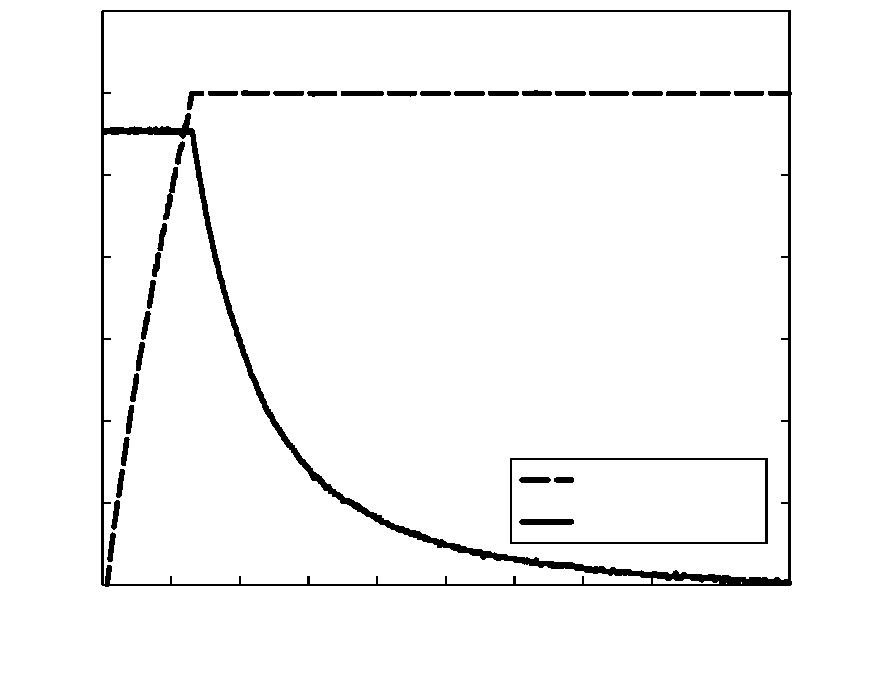
\includegraphics[width=\unitlength]{cur_lim_bonding}}%
        \put(0.91208943,0.09259998){\color[named]{black}\makebox(0,0)[lb]{\smash{0}}}%
        \put(0.91208943,0.18566494){\color[named]{black}\makebox(0,0)[lb]{\smash{0,5}}}%
        \put(0.91208943,0.27876279){\color[named]{black}\makebox(0,0)[lb]{\smash{1}}}%
        \put(0.91208943,0.37182771){\color[named]{black}\makebox(0,0)[lb]{\smash{1,5}}}%
        \put(0.91208943,0.46489266){\color[named]{black}\makebox(0,0)[lb]{\smash{2}}}%
        \put(0.91208943,0.55799055){\color[named]{black}\makebox(0,0)[lb]{\smash{2,5}}}%
        \put(0.91208943,0.65105543){\color[named]{black}\makebox(0,0)[lb]{\smash{3}}}%
        \put(0.91208943,0.74412039){\color[named]{black}\makebox(0,0)[lb]{\smash{3,5}}}%
        \put(0.10,0.09259998){\color[named]{black}\makebox(0,0)[rb]{\smash{400}}}%
        \put(0.10,0.18566494){\color[named]{black}\makebox(0,0)[rb]{\smash{500}}}%
        \put(0.10,0.27876279){\color[named]{black}\makebox(0,0)[rb]{\smash{600}}}%
        \put(0.10,0.37182771){\color[named]{black}\makebox(0,0)[rb]{\smash{700}}}%
        \put(0.10,0.46489266){\color[named]{black}\makebox(0,0)[rb]{\smash{800}}}%
        \put(0.10,0.55799055){\color[named]{black}\makebox(0,0)[rb]{\smash{900}}}%
        \put(0.10,0.65105543){\color[named]{black}\makebox(0,0)[rb]{\smash{1000}}}%
        \put(0.10,0.74412039){\color[named]{black}\makebox(0,0)[rb]{\smash{1100}}}%
        \put(0.11657128,0.055963){\color[named]{black}\makebox(0,0)[b]{\smash{0}}}%
        \put(0.19530171,0.055963){\color[named]{black}\makebox(0,0)[b]{\smash{3}}}%
        \put(0.27254373,0.055963){\color[named]{black}\makebox(0,0)[b]{\smash{6}}}%
        \put(0.35069174,0.055963){\color[named]{black}\makebox(0,0)[b]{\smash{9}}}%
        \put(0.42739995,0.055963){\color[named]{black}\makebox(0,0)[b]{\smash{12}}}%
        \put(0.50582292,0.055963){\color[named]{black}\makebox(0,0)[b]{\smash{15}}}%
        \put(0.58370406,0.055963){\color[named]{black}\makebox(0,0)[b]{\smash{18}}}%
        \put(0.66437591,0.055963){\color[named]{black}\makebox(0,0)[b]{\smash{21}}}%
        \put(0.74094652,0.055963){\color[named]{black}\makebox(0,0)[b]{\smash{24}}}%
        \put(0.81912689,0.055963){\color[named]{black}\makebox(0,0)[b]{\smash{27}}}%
        \put(0.89668439,0.055963){\color[named]{black}\makebox(0,0)[b]{\smash{30}}}%
        \put(1.01,0.4){\color[named]{black}\rotatebox{90}{\makebox(0,0)[b]{\smash{Ток, мА}}}}%
        \put(0.0,0.4){\color[named]{black}\rotatebox{90}{\makebox(0,0)[b]{\smash{Напряжение, В}}}}%
        \put(0.50676936,0.0070862){\color[named]{black}\makebox(0,0)[b]{\smash{Время, мин}}}%
        \put(0.65544289,0.21014445){\color[rgb]{0,0,0}\makebox(0,0)[lb]{\small\smash{Напряжение}}}%
        \put(0.65544289,0.16261668){\color[rgb]{0,0,0}\makebox(0,0)[lb]{\small\smash{Ток}}}%
      \end{picture}%
    \endgroup%

    \caption{Ток и напряжение в~процессе электростатического соединения в~режиме ограничения тока}
    \label{fig:current_limited_graph}
\end{figure}


\section{Снижение остаточных напряжений}
Помимо выбора оптимальной температуры соединения существуют работы,
показывающие, что за счёт термообработки, следующей непосредственно за процессом
соединения, возможно снизить возникающие остаточные напряжения. В
подразделе~\ref{chap_temp_inconsistence} описаны статьи, посвящённые работам по
управлению величиной прогиба соединённых пластин за счёт термообработки при
температурах от~450 до~560~{\textdegree}C. Согласно опубликованным материалам,
это возможно благодаря вязкоупругим свойствам стекла.

Автор данной диссертационной работы проводил  исследования влияния
термообработки на остаточные напряжения. Использовались кристаллы кремния
размером 4\(\,\times\,\)4~мм и толщиной 0,4~мм с вытравленной полостью. Они были
предварительно электростатически соединены с пьедесталами из~стекла ЛК5 толщиной
5~мм при температурах от 300 до 400~{\textdegree}C. Ширина обода контакта
кремния со стеклом составляла 0,7~мм. В некоторых стеклянных пьедесталах были
сформированы отверстия диаметром 2~мм.

Режимы последующей термообработки приведены на Рисунке~\ref{fig:annealing_results}.
Первый вариант термообработки "--- нагрев до температуры
(415\(\pm\)30)~{\textdegree}C, выдержка 60~минут и~затем неуправляемое охлаждение.
Второй вариант термообработки "--- нагрев до температуры
(440\(\pm\)30)~{\textdegree}C, выдержка 15 минут и затем управляемое охлаждение со
скоростью не превышающей 3~{\textdegree}C/мин. Охлаждение проводилось
до~температуры 200~{\textdegree}C, на которой проходила выдержка 30~минут. Затем
образцы охлаждались в неконтролируемом режиме.
Контроль и управление нагревом осуществлялось ПИД\nb-регулятором Термодат~13К2
на основании данных термопар типа ТХК или терморезисторов Honeywell
\mbox{HEL-707-T-0-12-00}.

Остаточные напряжения в стекле до и после термообработки измерялись
в~соответствии с процедурами, описанными в
подразделе~\ref{chap:measure_glass_stress} на полярископе\nb-поляриметре
ПКС\nb-250. Съём показаний с полярископа осуществляла
М.\,Г.~Лукоперова.
Результаты обработки измерений приведены на Рисунке~\ref{fig:annealing_results}.
Среднеарифметическое значение остаточных напряжений в стекле было снижено более
чем в два раза в каждом из вариантов термообработки.

\begin{figure}[!htb]
    \centering%
    \noindent%
    \ifdefmacro{\tikzsetnextfilename}{\tikzsetnextfilename{annealing_results_p1}}{}%
    \begin{tikzpicture}[x=1pt,y=1pt]
\definecolor{fillColor}{RGB}{255,255,255}
\path[use as bounding box,fill=fillColor] (0,0) rectangle (426.79,192.06);
\begin{scope}
\path[clip] (  0.00,  0.00) rectangle (213.40,192.06);
\definecolor{drawColor}{RGB}{255,255,255}

\path[draw=drawColor,line width= 0.6pt,line join=round,line cap=round,fill=fillColor] ( -0.00,  0.00) rectangle (213.40,192.06);
\end{scope}
\begin{scope}
\path[clip] ( 39.23, 29.60) rectangle (206.65,192.06);
\definecolor{fillColor}{RGB}{255,255,255}

\path[fill=fillColor] ( 39.23, 29.60) rectangle (206.65,192.06);
\definecolor{drawColor}{gray}{0.98}

\path[draw=drawColor,line width= 0.6pt,line join=round] ( 39.23, 48.78) --
	(206.65, 48.78);

\path[draw=drawColor,line width= 0.6pt,line join=round] ( 39.23, 80.97) --
	(206.65, 80.97);

\path[draw=drawColor,line width= 0.6pt,line join=round] ( 39.23,116.73) --
	(206.65,116.73);

\path[draw=drawColor,line width= 0.6pt,line join=round] ( 39.23,152.49) --
	(206.65,152.49);

\path[draw=drawColor,line width= 0.6pt,line join=round] ( 39.23,177.52) --
	(206.65,177.52);

\path[draw=drawColor,line width= 0.6pt,line join=round] ( 72.78, 29.60) --
	( 72.78,192.06);

\path[draw=drawColor,line width= 0.6pt,line join=round] (124.67, 29.60) --
	(124.67,192.06);

\path[draw=drawColor,line width= 0.6pt,line join=round] (176.56, 29.60) --
	(176.56,192.06);
\definecolor{drawColor}{gray}{0.80}

\path[draw=drawColor,line width= 0.3pt,line join=round] ( 39.23, 34.48) --
	(206.65, 34.48);

\path[draw=drawColor,line width= 0.3pt,line join=round] ( 39.23, 63.09) --
	(206.65, 63.09);

\path[draw=drawColor,line width= 0.3pt,line join=round] ( 39.23, 98.85) --
	(206.65, 98.85);

\path[draw=drawColor,line width= 0.3pt,line join=round] ( 39.23,134.61) --
	(206.65,134.61);

\path[draw=drawColor,line width= 0.3pt,line join=round] ( 39.23,170.37) --
	(206.65,170.37);

\path[draw=drawColor,line width= 0.3pt,line join=round] ( 39.23,184.67) --
	(206.65,184.67);

\path[draw=drawColor,line width= 0.3pt,line join=round] ( 46.84, 29.60) --
	( 46.84,192.06);

\path[draw=drawColor,line width= 0.3pt,line join=round] ( 98.72, 29.60) --
	( 98.72,192.06);

\path[draw=drawColor,line width= 0.3pt,line join=round] (150.61, 29.60) --
	(150.61,192.06);

\path[draw=drawColor,line width= 0.3pt,line join=round] (202.50, 29.60) --
	(202.50,192.06);
\definecolor{drawColor}{RGB}{0,0,0}

\path[draw=drawColor,line width= 1.3pt,line join=round] ( 46.84, 36.98) --
	( 47.34, 41.48) --
	( 47.85, 45.97) --
	( 48.35, 50.46) --
	( 48.85, 54.95) --
	( 49.36, 59.44) --
	( 49.86, 63.94) --
	( 50.37, 68.43) --
	( 50.87, 72.92) --
	( 51.37, 77.41) --
	( 51.88, 81.91) --
	( 52.38, 86.40) --
	( 52.89, 90.89) --
	( 53.39, 95.38) --
	( 53.89, 99.87) --
	( 54.40,104.37) --
	( 54.90,108.86) --
	( 55.40,113.35) --
	( 55.91,117.84) --
	( 56.41,122.34) --
	( 56.92,126.83) --
	( 57.42,131.32) --
	( 57.92,135.81) --
	( 58.43,140.30) --
	( 58.93,144.80) --
	( 59.44,149.29) --
	( 59.94,153.78) --
	( 60.44,158.27) --
	( 60.95,162.77) --
	( 61.45,167.26) --
	( 61.96,171.75) --
	( 62.46,175.73) --
	( 62.96,175.73) --
	( 63.47,175.73) --
	( 63.97,175.73) --
	( 64.48,175.73) --
	( 64.98,175.73) --
	( 65.48,175.73) --
	( 65.99,175.73) --
	( 66.49,175.73) --
	( 67.00,175.73) --
	( 67.50,175.73) --
	( 68.00,175.73) --
	( 68.51,175.73) --
	( 69.01,175.73) --
	( 69.52,175.73) --
	( 70.02,175.73) --
	( 70.52,175.73) --
	( 71.03,175.73) --
	( 71.53,175.73) --
	( 72.04,175.73) --
	( 72.54,175.73) --
	( 73.04,175.73) --
	( 73.55,175.73) --
	( 74.05,175.73) --
	( 74.56,175.73) --
	( 75.06,175.73) --
	( 75.56,175.73) --
	( 76.07,175.73) --
	( 76.57,175.73) --
	( 77.08,175.73) --
	( 77.58,175.73) --
	( 78.08,175.73) --
	( 78.59,175.73) --
	( 79.09,175.73) --
	( 79.60,175.73) --
	( 80.10,175.73) --
	( 80.60,175.73) --
	( 81.11,175.73) --
	( 81.61,175.73) --
	( 82.12,175.73) --
	( 82.62,175.73) --
	( 83.12,175.73) --
	( 83.63,175.73) --
	( 84.13,175.73) --
	( 84.64,175.73) --
	( 85.14,175.73) --
	( 85.64,175.73) --
	( 86.15,175.73) --
	( 86.65,175.73) --
	( 87.16,175.73) --
	( 87.66,175.73) --
	( 88.16,175.73) --
	( 88.67,175.73) --
	( 89.17,175.73) --
	( 89.68,175.73) --
	( 90.18,175.73) --
	( 90.68,175.73) --
	( 91.19,175.73) --
	( 91.69,175.73) --
	( 92.20,175.73) --
	( 92.70,175.73) --
	( 93.20,175.73) --
	( 93.71,175.73) --
	( 94.21,175.73) --
	( 94.72,175.73) --
	( 95.22,175.73) --
	( 95.72,175.73) --
	( 96.23,175.73) --
	( 96.73,175.73) --
	( 97.24,175.73) --
	( 97.74,175.73) --
	( 98.24,175.73) --
	( 98.75,175.73) --
	( 99.25,175.73) --
	( 99.76,175.73) --
	(100.26,175.73) --
	(100.76,175.73) --
	(101.27,175.73) --
	(101.77,175.73) --
	(102.28,175.73) --
	(102.78,175.73) --
	(103.28,175.73) --
	(103.79,175.73) --
	(104.29,175.73) --
	(104.80,175.73) --
	(105.30,175.73) --
	(105.80,175.73) --
	(106.31,175.73) --
	(106.81,175.73) --
	(107.32,175.73) --
	(107.82,175.73) --
	(108.32,175.73) --
	(108.83,175.73) --
	(109.33,175.73) --
	(109.84,175.73) --
	(110.34,175.73) --
	(110.84,175.73) --
	(111.35,175.73) --
	(111.85,175.73) --
	(112.36,175.73) --
	(112.86,175.73) --
	(113.36,175.73) --
	(113.87,175.73) --
	(114.37,175.08) --
	(114.88,171.02) --
	(115.38,167.05) --
	(115.88,163.18) --
	(116.39,159.40) --
	(116.89,155.70) --
	(117.39,152.10) --
	(117.90,148.58) --
	(118.40,145.15) --
	(118.91,141.81) --
	(119.41,138.54) --
	(119.91,135.36) --
	(120.42,132.26) --
	(120.92,129.24) --
	(121.43,126.29) --
	(121.93,123.43) --
	(122.43,120.63) --
	(122.94,117.91) --
	(123.44,115.26) --
	(123.95,112.68) --
	(124.45,110.18) --
	(124.95,107.74) --
	(125.46,105.36) --
	(125.96,103.06) --
	(126.47,100.82) --
	(126.97, 98.64) --
	(127.47, 96.52) --
	(127.98, 94.47) --
	(128.48, 92.47) --
	(128.99, 90.53) --
	(129.49, 88.66) --
	(129.99, 86.83) --
	(130.50, 85.06) --
	(131.00, 83.35) --
	(131.51, 81.69) --
	(132.01, 80.08) --
	(132.51, 78.52) --
	(133.02, 77.02) --
	(133.52, 75.56) --
	(134.03, 74.14) --
	(134.53, 72.78) --
	(135.03, 71.46) --
	(135.54, 70.18) --
	(136.04, 68.95) --
	(136.55, 67.76) --
	(137.05, 66.61) --
	(137.55, 65.51) --
	(138.06, 64.44) --
	(138.56, 63.41) --
	(139.07, 62.42) --
	(139.57, 61.46) --
	(140.07, 60.54) --
	(140.58, 59.66) --
	(141.08, 58.81) --
	(141.59, 57.99) --
	(142.09, 57.20) --
	(142.59, 56.45) --
	(143.10, 55.73) --
	(143.60, 55.03) --
	(144.11, 54.37) --
	(144.61, 53.73) --
	(145.11, 53.12) --
	(145.62, 52.54) --
	(146.12, 51.98) --
	(146.63, 51.45) --
	(147.13, 50.94) --
	(147.63, 50.46) --
	(148.14, 50.00) --
	(148.64, 49.56) --
	(149.15, 49.14) --
	(149.65, 48.74) --
	(150.15, 48.36) --
	(150.66, 48.00) --
	(151.16, 47.66) --
	(151.67, 47.34) --
	(152.17, 47.04) --
	(152.67, 46.75) --
	(153.18, 46.47) --
	(153.68, 46.22) --
	(154.19, 45.97) --
	(154.69, 45.75) --
	(155.19, 45.53) --
	(155.70, 45.33) --
	(156.20, 45.14) --
	(156.71, 44.97) --
	(157.21, 44.80) --
	(157.71, 44.65) --
	(158.22, 44.50) --
	(158.72, 44.37) --
	(159.23, 44.24) --
	(159.73, 44.13) --
	(160.23, 44.02) --
	(160.74, 43.92) --
	(161.24, 43.83) --
	(161.75, 43.75) --
	(162.25, 43.67) --
	(162.75, 43.60) --
	(163.26, 43.54) --
	(163.76, 43.48) --
	(164.27, 43.43) --
	(164.77, 43.38) --
	(165.27, 43.34) --
	(165.78, 43.30);

\path[draw=drawColor,line width= 0.9pt,line join=round,line cap=round] ( 39.23, 29.60) rectangle (206.65,192.06);
\end{scope}
\begin{scope}
\path[clip] (  0.00,  0.00) rectangle (426.79,192.06);
\definecolor{drawColor}{RGB}{0,0,0}

\node[text=drawColor,anchor=base east,inner sep=0pt, outer sep=0pt, scale=  0.86] at ( 33.83, 30.23) {\(20\)};

\node[text=drawColor,anchor=base east,inner sep=0pt, outer sep=0pt, scale=  0.86] at ( 33.83, 58.84) {\(100\)};

\node[text=drawColor,anchor=base east,inner sep=0pt, outer sep=0pt, scale=  0.86] at ( 33.83, 94.60) {\(200\)};

\node[text=drawColor,anchor=base east,inner sep=0pt, outer sep=0pt, scale=  0.86] at ( 33.83,130.36) {\(300\)};

\node[text=drawColor,anchor=base east,inner sep=0pt, outer sep=0pt, scale=  0.86] at ( 33.83,166.12) {\(400\)};

\node[text=drawColor,anchor=base east,inner sep=0pt, outer sep=0pt, scale=  0.86] at ( 33.83,180.42) {\(440\)};
\end{scope}
\begin{scope}
\path[clip] (  0.00,  0.00) rectangle (426.79,192.06);
\definecolor{drawColor}{RGB}{0,0,0}

\path[draw=drawColor,line width= 0.6pt,line join=round] ( 36.23, 34.48) --
	( 39.23, 34.48);

\path[draw=drawColor,line width= 0.6pt,line join=round] ( 36.23, 63.09) --
	( 39.23, 63.09);

\path[draw=drawColor,line width= 0.6pt,line join=round] ( 36.23, 98.85) --
	( 39.23, 98.85);

\path[draw=drawColor,line width= 0.6pt,line join=round] ( 36.23,134.61) --
	( 39.23,134.61);

\path[draw=drawColor,line width= 0.6pt,line join=round] ( 36.23,170.37) --
	( 39.23,170.37);

\path[draw=drawColor,line width= 0.6pt,line join=round] ( 36.23,184.67) --
	( 39.23,184.67);
\end{scope}
\begin{scope}
\path[clip] (  0.00,  0.00) rectangle (426.79,192.06);
\definecolor{drawColor}{RGB}{0,0,0}

\path[draw=drawColor,line width= 0.6pt,line join=round] ( 46.84, 26.60) --
	( 46.84, 29.60);

\path[draw=drawColor,line width= 0.6pt,line join=round] ( 98.72, 26.60) --
	( 98.72, 29.60);

\path[draw=drawColor,line width= 0.6pt,line join=round] (150.61, 26.60) --
	(150.61, 29.60);

\path[draw=drawColor,line width= 0.6pt,line join=round] (202.50, 26.60) --
	(202.50, 29.60);
\end{scope}
\begin{scope}
\path[clip] (  0.00,  0.00) rectangle (426.79,192.06);
\definecolor{drawColor}{RGB}{0,0,0}

\node[text=drawColor,anchor=base,inner sep=0pt, outer sep=0pt, scale=  0.86] at ( 46.84, 15.70) {\(0\)};

\node[text=drawColor,anchor=base,inner sep=0pt, outer sep=0pt, scale=  0.86] at ( 98.72, 15.70) {\(60\)};

\node[text=drawColor,anchor=base,inner sep=0pt, outer sep=0pt, scale=  0.86] at (150.61, 15.70) {\(120\)};

\node[text=drawColor,anchor=base,inner sep=0pt, outer sep=0pt, scale=  0.86] at (202.50, 15.70) {\(180\)};
\end{scope}
\begin{scope}
\path[clip] (  0.00,  0.00) rectangle (426.79,192.06);
\definecolor{drawColor}{RGB}{0,0,0}

\node[text=drawColor,anchor=base,inner sep=0pt, outer sep=0pt, scale=  0.86] at (122.94,  2.40) {Время, мин};
\end{scope}
\begin{scope}
\path[clip] (  0.00,  0.00) rectangle (426.79,192.06);
\definecolor{drawColor}{RGB}{0,0,0}

\node[text=drawColor,rotate= 90.00,anchor=base,inner sep=0pt, outer sep=0pt, scale=  0.86] at ( 10.90,110.83) {Tемпература, \({}^\circ\)C\hspace*{1.7em}};
\end{scope}
\begin{scope}
\path[clip] (213.40,  0.00) rectangle (426.79,192.06);
\definecolor{drawColor}{RGB}{255,255,255}
\definecolor{fillColor}{RGB}{255,255,255}

\path[draw=drawColor,line width= 0.6pt,line join=round,line cap=round,fill=fillColor] (213.40,  0.00) rectangle (426.79,192.06);
\end{scope}
\begin{scope}
\path[clip] (252.62, 29.60) rectangle (420.05,192.06);
\definecolor{fillColor}{RGB}{255,255,255}

\path[fill=fillColor] (252.62, 29.60) rectangle (420.05,192.06);
\definecolor{drawColor}{gray}{0.98}

\path[draw=drawColor,line width= 0.6pt,line join=round] (252.62, 48.78) --
	(420.05, 48.78);

\path[draw=drawColor,line width= 0.6pt,line join=round] (252.62, 80.97) --
	(420.05, 80.97);

\path[draw=drawColor,line width= 0.6pt,line join=round] (252.62,116.73) --
	(420.05,116.73);

\path[draw=drawColor,line width= 0.6pt,line join=round] (252.62,152.49) --
	(420.05,152.49);

\path[draw=drawColor,line width= 0.6pt,line join=round] (252.62,177.52) --
	(420.05,177.52);

\path[draw=drawColor,line width= 0.6pt,line join=round] (286.18, 29.60) --
	(286.18,192.06);

\path[draw=drawColor,line width= 0.6pt,line join=round] (338.06, 29.60) --
	(338.06,192.06);

\path[draw=drawColor,line width= 0.6pt,line join=round] (389.95, 29.60) --
	(389.95,192.06);
\definecolor{drawColor}{gray}{0.80}

\path[draw=drawColor,line width= 0.3pt,line join=round] (252.62, 34.48) --
	(420.05, 34.48);

\path[draw=drawColor,line width= 0.3pt,line join=round] (252.62, 63.09) --
	(420.05, 63.09);

\path[draw=drawColor,line width= 0.3pt,line join=round] (252.62, 98.85) --
	(420.05, 98.85);

\path[draw=drawColor,line width= 0.3pt,line join=round] (252.62,134.61) --
	(420.05,134.61);

\path[draw=drawColor,line width= 0.3pt,line join=round] (252.62,170.37) --
	(420.05,170.37);

\path[draw=drawColor,line width= 0.3pt,line join=round] (252.62,184.67) --
	(420.05,184.67);

\path[draw=drawColor,line width= 0.3pt,line join=round] (260.23, 29.60) --
	(260.23,192.06);

\path[draw=drawColor,line width= 0.3pt,line join=round] (312.12, 29.60) --
	(312.12,192.06);

\path[draw=drawColor,line width= 0.3pt,line join=round] (364.01, 29.60) --
	(364.01,192.06);

\path[draw=drawColor,line width= 0.3pt,line join=round] (415.90, 29.60) --
	(415.90,192.06);
\definecolor{drawColor}{RGB}{0,0,0}

\path[draw=drawColor,line width= 1.3pt,line join=round] (260.23, 36.98) --
	(260.74, 42.05) --
	(261.24, 47.11) --
	(261.74, 52.17) --
	(262.25, 57.24) --
	(262.75, 62.30) --
	(263.26, 67.36) --
	(263.76, 72.42) --
	(264.26, 77.49) --
	(264.77, 82.55) --
	(265.27, 87.61) --
	(265.78, 92.68) --
	(266.28, 97.74) --
	(266.78,102.80) --
	(267.29,107.86) --
	(267.79,112.93) --
	(268.30,117.99) --
	(268.80,123.05) --
	(269.30,128.12) --
	(269.81,133.18) --
	(270.31,138.24) --
	(270.82,143.31) --
	(271.32,148.37) --
	(271.82,153.43) --
	(272.33,158.49) --
	(272.83,163.56) --
	(273.34,168.62) --
	(273.84,173.68) --
	(274.34,178.75) --
	(274.85,183.81) --
	(275.35,184.67) --
	(275.86,184.67) --
	(276.36,184.67) --
	(276.86,184.67) --
	(277.37,184.67) --
	(277.87,184.67) --
	(278.38,184.67) --
	(278.88,184.67) --
	(279.38,184.67) --
	(279.89,184.67) --
	(280.39,184.67) --
	(280.90,184.67) --
	(281.40,184.67) --
	(281.90,184.67) --
	(282.41,184.67) --
	(282.91,184.67) --
	(283.42,184.67) --
	(283.92,184.67) --
	(284.42,184.67) --
	(284.93,184.67) --
	(285.43,184.67) --
	(285.94,184.67) --
	(286.44,184.67) --
	(286.94,184.67) --
	(287.45,184.67) --
	(287.95,184.67) --
	(288.46,184.67) --
	(288.96,184.67) --
	(289.46,184.67) --
	(289.97,184.67) --
	(290.47,184.67) --
	(290.98,184.08) --
	(291.48,183.46) --
	(291.98,182.83) --
	(292.49,182.21) --
	(292.99,181.58) --
	(293.50,180.96) --
	(294.00,180.33) --
	(294.50,179.71) --
	(295.01,179.08) --
	(295.51,178.46) --
	(296.02,177.83) --
	(296.52,177.20) --
	(297.02,176.58) --
	(297.53,175.95) --
	(298.03,175.33) --
	(298.54,174.70) --
	(299.04,174.08) --
	(299.54,173.45) --
	(300.05,172.83) --
	(300.55,172.20) --
	(301.06,171.58) --
	(301.56,170.95) --
	(302.06,170.33) --
	(302.57,169.70) --
	(303.07,169.08) --
	(303.58,168.45) --
	(304.08,167.83) --
	(304.58,167.20) --
	(305.09,166.58) --
	(305.59,165.95) --
	(306.10,165.33) --
	(306.60,164.70) --
	(307.10,164.08) --
	(307.61,163.45) --
	(308.11,162.83) --
	(308.62,162.20) --
	(309.12,161.57) --
	(309.62,160.95) --
	(310.13,160.32) --
	(310.63,159.70) --
	(311.14,159.07) --
	(311.64,158.45) --
	(312.14,157.82) --
	(312.65,157.20) --
	(313.15,156.57) --
	(313.66,155.95) --
	(314.16,155.32) --
	(314.66,154.70) --
	(315.17,154.07) --
	(315.67,153.45) --
	(316.18,152.82) --
	(316.68,152.20) --
	(317.18,151.57) --
	(317.69,150.95) --
	(318.19,150.32) --
	(318.70,149.70) --
	(319.20,149.07) --
	(319.70,148.45) --
	(320.21,147.82) --
	(320.71,147.19) --
	(321.21,146.57) --
	(321.72,145.94) --
	(322.22,145.32) --
	(322.73,144.69) --
	(323.23,144.07) --
	(323.73,143.44) --
	(324.24,142.82) --
	(324.74,142.19) --
	(325.25,141.57) --
	(325.75,140.94) --
	(326.25,140.32) --
	(326.76,139.69) --
	(327.26,139.07) --
	(327.77,138.44) --
	(328.27,137.82) --
	(328.77,137.19) --
	(329.28,136.57) --
	(329.78,135.94) --
	(330.29,135.32) --
	(330.79,134.69) --
	(331.29,134.07) --
	(331.80,133.44) --
	(332.30,132.82) --
	(332.81,132.19) --
	(333.31,131.56) --
	(333.81,130.94) --
	(334.32,130.31) --
	(334.82,129.69) --
	(335.33,129.06) --
	(335.83,128.44) --
	(336.33,127.81) --
	(336.84,127.19) --
	(337.34,126.56) --
	(337.85,125.94) --
	(338.35,125.31) --
	(338.85,124.69) --
	(339.36,124.06) --
	(339.86,123.44) --
	(340.37,122.81) --
	(340.87,122.19) --
	(341.37,121.56) --
	(341.88,120.94) --
	(342.38,120.31) --
	(342.89,119.69) --
	(343.39,119.06) --
	(343.89,118.44) --
	(344.40,117.81) --
	(344.90,117.19) --
	(345.41,116.56) --
	(345.91,115.93) --
	(346.41,115.31) --
	(346.92,114.68) --
	(347.42,114.06) --
	(347.93,113.43) --
	(348.43,112.81) --
	(348.93,112.18) --
	(349.44,111.56) --
	(349.94,110.93) --
	(350.45,110.31) --
	(350.95,109.68) --
	(351.45,109.06) --
	(351.96,108.43) --
	(352.46,107.81) --
	(352.97,107.18) --
	(353.47,106.56) --
	(353.97,105.93) --
	(354.48,105.31) --
	(354.98,104.68) --
	(355.49,104.06) --
	(355.99,103.43) --
	(356.49,102.81) --
	(357.00,102.18) --
	(357.50,101.55) --
	(358.01,100.93) --
	(358.51,100.30) --
	(359.01, 99.68) --
	(359.52, 99.05) --
	(360.02, 98.85) --
	(360.53, 98.85) --
	(361.03, 98.85) --
	(361.53, 98.85) --
	(362.04, 98.85) --
	(362.54, 98.85) --
	(363.05, 98.85) --
	(363.55, 98.85) --
	(364.05, 98.85) --
	(364.56, 98.85) --
	(365.06, 98.85) --
	(365.57, 98.85) --
	(366.07, 98.85) --
	(366.57, 98.85) --
	(367.08, 98.85) --
	(367.58, 98.85) --
	(368.09, 98.85) --
	(368.59, 98.85) --
	(369.09, 98.85) --
	(369.60, 98.85) --
	(370.10, 98.85) --
	(370.61, 98.85) --
	(371.11, 98.85) --
	(371.61, 98.85) --
	(372.12, 98.85) --
	(372.62, 98.85) --
	(373.13, 98.85) --
	(373.63, 98.85) --
	(374.13, 98.85) --
	(374.64, 98.85) --
	(375.14, 98.85) --
	(375.65, 98.85) --
	(376.15, 98.85) --
	(376.65, 98.85) --
	(377.16, 98.85) --
	(377.66, 98.85) --
	(378.17, 98.85) --
	(378.67, 98.85) --
	(379.17, 98.85) --
	(379.68, 98.85) --
	(380.18, 98.85) --
	(380.69, 98.85) --
	(381.19, 98.85) --
	(381.69, 98.85) --
	(382.20, 98.72) --
	(382.70, 96.51) --
	(383.20, 94.36) --
	(383.71, 92.27) --
	(384.21, 90.24) --
	(384.72, 88.28) --
	(385.22, 86.37) --
	(385.72, 84.52) --
	(386.23, 82.73) --
	(386.73, 81.00) --
	(387.24, 79.32) --
	(387.74, 77.69) --
	(388.24, 76.12) --
	(388.75, 74.59) --
	(389.25, 73.12) --
	(389.76, 71.70) --
	(390.26, 70.32) --
	(390.76, 68.99) --
	(391.27, 67.70) --
	(391.77, 66.46) --
	(392.28, 65.27) --
	(392.78, 64.11) --
	(393.28, 63.00) --
	(393.79, 61.93) --
	(394.29, 60.90) --
	(394.80, 59.90) --
	(395.30, 58.95) --
	(395.80, 58.03) --
	(396.31, 57.14) --
	(396.81, 56.29) --
	(397.32, 55.48) --
	(397.82, 54.70) --
	(398.32, 53.94) --
	(398.83, 53.23) --
	(399.33, 52.54) --
	(399.84, 51.88) --
	(400.34, 51.24) --
	(400.84, 50.64) --
	(401.35, 50.06) --
	(401.85, 49.51) --
	(402.36, 48.99) --
	(402.86, 48.49) --
	(403.36, 48.01) --
	(403.87, 47.55) --
	(404.37, 47.12) --
	(404.88, 46.71) --
	(405.38, 46.32) --
	(405.88, 45.95) --
	(406.39, 45.60) --
	(406.89, 45.27) --
	(407.40, 44.95) --
	(407.90, 44.66) --
	(408.40, 44.38) --
	(408.91, 44.11) --
	(409.41, 43.86) --
	(409.92, 43.63) --
	(410.42, 43.41) --
	(410.92, 43.21) --
	(411.43, 43.01) --
	(411.93, 42.83) --
	(412.44, 42.66);

\path[draw=drawColor,line width= 0.9pt,line join=round,line cap=round] (252.62, 29.60) rectangle (420.05,192.06);
\end{scope}
\begin{scope}
\path[clip] (  0.00,  0.00) rectangle (426.79,192.06);
\definecolor{drawColor}{RGB}{0,0,0}

\node[text=drawColor,anchor=base east,inner sep=0pt, outer sep=0pt, scale=  0.86] at (247.22, 30.23) {\(20\)};

\node[text=drawColor,anchor=base east,inner sep=0pt, outer sep=0pt, scale=  0.86] at (247.22, 58.84) {\(100\)};

\node[text=drawColor,anchor=base east,inner sep=0pt, outer sep=0pt, scale=  0.86] at (247.22, 94.60) {\(200\)};

\node[text=drawColor,anchor=base east,inner sep=0pt, outer sep=0pt, scale=  0.86] at (247.22,130.36) {\(300\)};

\node[text=drawColor,anchor=base east,inner sep=0pt, outer sep=0pt, scale=  0.86] at (247.22,166.12) {\(400\)};

\node[text=drawColor,anchor=base east,inner sep=0pt, outer sep=0pt, scale=  0.86] at (247.22,180.42) {\(440\)};
\end{scope}
\begin{scope}
\path[clip] (  0.00,  0.00) rectangle (426.79,192.06);
\definecolor{drawColor}{RGB}{0,0,0}

\path[draw=drawColor,line width= 0.6pt,line join=round] (249.62, 34.48) --
	(252.62, 34.48);

\path[draw=drawColor,line width= 0.6pt,line join=round] (249.62, 63.09) --
	(252.62, 63.09);

\path[draw=drawColor,line width= 0.6pt,line join=round] (249.62, 98.85) --
	(252.62, 98.85);

\path[draw=drawColor,line width= 0.6pt,line join=round] (249.62,134.61) --
	(252.62,134.61);

\path[draw=drawColor,line width= 0.6pt,line join=round] (249.62,170.37) --
	(252.62,170.37);

\path[draw=drawColor,line width= 0.6pt,line join=round] (249.62,184.67) --
	(252.62,184.67);
\end{scope}
\begin{scope}
\path[clip] (  0.00,  0.00) rectangle (426.79,192.06);
\definecolor{drawColor}{RGB}{0,0,0}

\path[draw=drawColor,line width= 0.6pt,line join=round] (260.23, 26.60) --
	(260.23, 29.60);

\path[draw=drawColor,line width= 0.6pt,line join=round] (312.12, 26.60) --
	(312.12, 29.60);

\path[draw=drawColor,line width= 0.6pt,line join=round] (364.01, 26.60) --
	(364.01, 29.60);

\path[draw=drawColor,line width= 0.6pt,line join=round] (415.90, 26.60) --
	(415.90, 29.60);
\end{scope}
\begin{scope}
\path[clip] (  0.00,  0.00) rectangle (426.79,192.06);
\definecolor{drawColor}{RGB}{0,0,0}

\node[text=drawColor,anchor=base,inner sep=0pt, outer sep=0pt, scale=  0.86] at (260.23, 15.70) {\(0\)};

\node[text=drawColor,anchor=base,inner sep=0pt, outer sep=0pt, scale=  0.86] at (312.12, 15.70) {\(60\)};

\node[text=drawColor,anchor=base,inner sep=0pt, outer sep=0pt, scale=  0.86] at (364.01, 15.70) {\(120\)};

\node[text=drawColor,anchor=base,inner sep=0pt, outer sep=0pt, scale=  0.86] at (415.90, 15.70) {\(180\)};
\end{scope}
\begin{scope}
\path[clip] (  0.00,  0.00) rectangle (426.79,192.06);
\definecolor{drawColor}{RGB}{0,0,0}

\node[text=drawColor,anchor=base,inner sep=0pt, outer sep=0pt, scale=  0.86] at (336.33,  2.40) {Время, мин};
\end{scope}
\begin{scope}
\path[clip] (  0.00,  0.00) rectangle (426.79,192.06);
\definecolor{drawColor}{RGB}{0,0,0}

\node[text=drawColor,rotate= 90.00,anchor=base,inner sep=0pt, outer sep=0pt, scale=  0.86] at (224.30,110.83) {Tемпература, \({}^\circ\)C\hspace*{1.7em}};
\end{scope}
\end{tikzpicture}
%
    \par%
    \noindent%
    \ifdefmacro{\tikzsetnextfilename}{\tikzsetnextfilename{annealing_results_p2}}{}%
    \begin{tikzpicture}[x=1pt,y=1pt]
\definecolor{fillColor}{RGB}{255,255,255}
\path[use as bounding box,fill=fillColor] (0,0) rectangle (426.79,213.40);
\begin{scope}
\path[clip] (  0.00,  0.00) rectangle (426.79,213.40);
\definecolor{drawColor}{RGB}{255,255,255}

\path[draw=drawColor,line width= 0.6pt,line join=round,line cap=round,fill=fillColor] (  0.00,  0.00) rectangle (426.79,213.40);
\end{scope}
\begin{scope}
\path[clip] ( 39.98, 31.05) rectangle (226.17,195.49);
\definecolor{fillColor}{RGB}{255,255,255}

\path[fill=fillColor] ( 39.98, 31.05) rectangle (226.17,195.49);
\definecolor{drawColor}{gray}{0.98}

\path[draw=drawColor,line width= 0.6pt,line join=round] ( 39.98, 56.57) --
	(226.17, 56.57);

\path[draw=drawColor,line width= 0.6pt,line join=round] ( 39.98, 92.66) --
	(226.17, 92.66);

\path[draw=drawColor,line width= 0.6pt,line join=round] ( 39.98,128.75) --
	(226.17,128.75);

\path[draw=drawColor,line width= 0.6pt,line join=round] ( 39.98,164.84) --
	(226.17,164.84);
\definecolor{drawColor}{gray}{0.80}

\path[draw=drawColor,line width= 0.3pt,line join=round] ( 39.98, 38.52) --
	(226.17, 38.52);

\path[draw=drawColor,line width= 0.3pt,line join=round] ( 39.98, 74.61) --
	(226.17, 74.61);

\path[draw=drawColor,line width= 0.3pt,line join=round] ( 39.98,110.70) --
	(226.17,110.70);

\path[draw=drawColor,line width= 0.3pt,line join=round] ( 39.98,146.80) --
	(226.17,146.80);

\path[draw=drawColor,line width= 0.3pt,line join=round] ( 39.98,182.89) --
	(226.17,182.89);

\path[draw=drawColor,line width= 0.3pt,line join=round] ( 90.76, 31.05) --
	( 90.76,195.49);

\path[draw=drawColor,line width= 0.3pt,line join=round] (175.39, 31.05) --
	(175.39,195.49);
\definecolor{fillColor}{RGB}{128,128,128}

\path[fill=fillColor] ( 52.67, 38.52) rectangle (128.84,134.68);
\definecolor{fillColor}{gray}{0.80}

\path[fill=fillColor] (137.30, 38.52) rectangle (213.47, 83.94);
\definecolor{drawColor}{RGB}{0,0,0}

\node[text=drawColor,anchor=base,inner sep=0pt, outer sep=0pt, scale=  1.00] at ( 90.76, 81.62) {100 \%};

\node[text=drawColor,anchor=base,inner sep=0pt, outer sep=0pt, scale=  1.00] at (175.39, 56.25) {47 \%};

\path[draw=drawColor,line width= 0.9pt,line join=round,line cap=round] ( 39.98, 31.05) rectangle (226.17,195.49);
\end{scope}
\begin{scope}
\path[clip] (232.17, 31.05) rectangle (418.36,195.49);
\definecolor{fillColor}{RGB}{255,255,255}

\path[fill=fillColor] (232.17, 31.05) rectangle (418.36,195.49);
\definecolor{drawColor}{gray}{0.98}

\path[draw=drawColor,line width= 0.6pt,line join=round] (232.17, 56.57) --
	(418.36, 56.57);

\path[draw=drawColor,line width= 0.6pt,line join=round] (232.17, 92.66) --
	(418.36, 92.66);

\path[draw=drawColor,line width= 0.6pt,line join=round] (232.17,128.75) --
	(418.36,128.75);

\path[draw=drawColor,line width= 0.6pt,line join=round] (232.17,164.84) --
	(418.36,164.84);
\definecolor{drawColor}{gray}{0.80}

\path[draw=drawColor,line width= 0.3pt,line join=round] (232.17, 38.52) --
	(418.36, 38.52);

\path[draw=drawColor,line width= 0.3pt,line join=round] (232.17, 74.61) --
	(418.36, 74.61);

\path[draw=drawColor,line width= 0.3pt,line join=round] (232.17,110.70) --
	(418.36,110.70);

\path[draw=drawColor,line width= 0.3pt,line join=round] (232.17,146.80) --
	(418.36,146.80);

\path[draw=drawColor,line width= 0.3pt,line join=round] (232.17,182.89) --
	(418.36,182.89);

\path[draw=drawColor,line width= 0.3pt,line join=round] (282.95, 31.05) --
	(282.95,195.49);

\path[draw=drawColor,line width= 0.3pt,line join=round] (367.58, 31.05) --
	(367.58,195.49);
\definecolor{fillColor}{RGB}{128,128,128}

\path[fill=fillColor] (244.86, 38.52) rectangle (321.03,188.02);
\definecolor{fillColor}{gray}{0.80}

\path[fill=fillColor] (329.50, 38.52) rectangle (405.66,104.99);
\definecolor{drawColor}{RGB}{0,0,0}

\node[text=drawColor,anchor=base,inner sep=0pt, outer sep=0pt, scale=  1.00] at (282.95,108.29) {100 \%};

\node[text=drawColor,anchor=base,inner sep=0pt, outer sep=0pt, scale=  1.00] at (367.58, 66.78) {44 \%};

\path[draw=drawColor,line width= 0.9pt,line join=round,line cap=round] (232.17, 31.05) rectangle (418.36,195.49);
\end{scope}
\begin{scope}
\path[clip] ( 39.98,195.49) rectangle (226.17,210.02);
\definecolor{drawColor}{gray}{0.40}
\definecolor{fillColor}{gray}{0.90}

\path[draw=drawColor,line width= 0.9pt,line join=round,line cap=round,fill=fillColor] ( 39.98,195.49) rectangle (226.17,210.02);
\definecolor{drawColor}{gray}{0.10}

\node[text=drawColor,anchor=base,inner sep=0pt, outer sep=0pt, scale=  0.86] at (133.07,198.49) {Выдержка 415 \({}^\circ\)C 60 мин};
\end{scope}
\begin{scope}
\path[clip] (232.17,195.49) rectangle (418.36,210.02);
\definecolor{drawColor}{gray}{0.40}
\definecolor{fillColor}{gray}{0.90}

\path[draw=drawColor,line width= 0.9pt,line join=round,line cap=round,fill=fillColor] (232.17,195.49) rectangle (418.36,210.02);
\definecolor{drawColor}{gray}{0.10}

\node[text=drawColor,anchor=base,inner sep=0pt, outer sep=0pt, scale=  0.86] at (325.26,198.49) {Выдержка 440 \({}^\circ\)C 15 мин};
\end{scope}
\begin{scope}
\path[clip] (  0.00,  0.00) rectangle (426.79,213.40);
\definecolor{drawColor}{RGB}{0,0,0}

\node[text=drawColor,anchor=base east,inner sep=0pt, outer sep=0pt, scale=  0.86] at ( 34.58, 34.26) {0};

\node[text=drawColor,anchor=base east,inner sep=0pt, outer sep=0pt, scale=  0.86] at ( 34.58, 70.35) {0,2};

\node[text=drawColor,anchor=base east,inner sep=0pt, outer sep=0pt, scale=  0.86] at ( 34.58,106.44) {0,4};

\node[text=drawColor,anchor=base east,inner sep=0pt, outer sep=0pt, scale=  0.86] at ( 34.58,142.53) {0,6};

\node[text=drawColor,anchor=base east,inner sep=0pt, outer sep=0pt, scale=  0.86] at ( 34.58,178.62) {0,8};
\end{scope}
\begin{scope}
\path[clip] (  0.00,  0.00) rectangle (426.79,213.40);
\definecolor{drawColor}{RGB}{0,0,0}

\path[draw=drawColor,line width= 0.6pt,line join=round] ( 36.98, 38.52) --
	( 39.98, 38.52);

\path[draw=drawColor,line width= 0.6pt,line join=round] ( 36.98, 74.61) --
	( 39.98, 74.61);

\path[draw=drawColor,line width= 0.6pt,line join=round] ( 36.98,110.70) --
	( 39.98,110.70);

\path[draw=drawColor,line width= 0.6pt,line join=round] ( 36.98,146.80) --
	( 39.98,146.80);

\path[draw=drawColor,line width= 0.6pt,line join=round] ( 36.98,182.89) --
	( 39.98,182.89);
\end{scope}
\begin{scope}
\path[clip] (  0.00,  0.00) rectangle (426.79,213.40);
\definecolor{drawColor}{RGB}{0,0,0}

\path[draw=drawColor,line width= 0.6pt,line join=round] ( 90.76, 28.05) --
	( 90.76, 31.05);

\path[draw=drawColor,line width= 0.6pt,line join=round] (175.39, 28.05) --
	(175.39, 31.05);
\end{scope}
\begin{scope}
\path[clip] (  0.00,  0.00) rectangle (426.79,213.40);
\definecolor{drawColor}{RGB}{0,0,0}

\node[text=drawColor,anchor=base,inner sep=0pt, outer sep=0pt, scale=  0.86] at ( 90.76, 17.12) {Нет};

\node[text=drawColor,anchor=base,inner sep=0pt, outer sep=0pt, scale=  0.86] at (175.39, 17.12) {Да};
\end{scope}
\begin{scope}
\path[clip] (  0.00,  0.00) rectangle (426.79,213.40);
\definecolor{drawColor}{RGB}{0,0,0}

\path[draw=drawColor,line width= 0.6pt,line join=round] (282.95, 28.05) --
	(282.95, 31.05);

\path[draw=drawColor,line width= 0.6pt,line join=round] (367.58, 28.05) --
	(367.58, 31.05);
\end{scope}
\begin{scope}
\path[clip] (  0.00,  0.00) rectangle (426.79,213.40);
\definecolor{drawColor}{RGB}{0,0,0}

\node[text=drawColor,anchor=base,inner sep=0pt, outer sep=0pt, scale=  0.86] at (282.95, 17.12) {Нет};

\node[text=drawColor,anchor=base,inner sep=0pt, outer sep=0pt, scale=  0.86] at (367.58, 17.12) {Да};
\end{scope}
\begin{scope}
\path[clip] (  0.00,  0.00) rectangle (426.79,213.40);
\definecolor{drawColor}{RGB}{0,0,0}

\node[text=drawColor,anchor=base,inner sep=0pt, outer sep=0pt, scale=  1.00] at (229.17,  2.40) {Термообработка};
\end{scope}
\begin{scope}
\path[clip] (  0.00,  0.00) rectangle (426.79,213.40);
\definecolor{drawColor}{RGB}{0,0,0}

\node[text=drawColor,rotate= 90.00,anchor=base,inner sep=0pt, outer sep=0pt, scale=  1.00] at ( 12.32,113.27) {Напряжение, МПа\hspace*{1.5em}};
\end{scope}
\end{tikzpicture}
%
    \par%

    \caption{Снижение остаточных напряжений термообработкой}
    \label{fig:annealing_results}
\end{figure}

Были проведены исследования возможности снижения остаточных напряжений в
процессе остывания сборок непосредственно по окончании процесса, за~счёт
контролируемой скорости охлаждения. По сравнению с отдельной термообработкой
происходит выигрыш во времени на охлаждение после процесса и~дальнейший нагрев с
выдержкой, но используется более щадящий режим охлаждения.

Исследовалось влияние контролируемого охлаждения со скоростью не~выше
2~{\textdegree}C/мин сразу после окончания подачи высокого напряжения
до~температуры 200~{\textdegree}C, а затем неуправляемого охлаждения. Ограничением
такого способа является снижение его потенциального воздействия со снижением
температуры проведения процесса.

На Рисунке~\ref{fig:cooling_control_temp} приведена кривая исследованного
процесса управляемого охлаждения. Образцы, аналогичные исследовавшимся при
отдельной термообработке, выдерживались не менее 15 минут при температуре
(440$\pm$30)~{\textdegree}C, затем проводилось электростатическое соединение,
занимавшее от 10 до 15~минут. По~окончании подачи высокого напряжения начиналось
контролируемое охлаждение со~скоростью не выше 2~{\textdegree}C/мин до
200~{\textdegree}C, после чего охлаждением не~управляли.

\begin{figure}[!htb]
    \centering%
    \noindent%
    \ifdefmacro{\tikzsetnextfilename}{\tikzsetnextfilename{cooling_control_temp_p1}}{}%
    \begin{tikzpicture}[x=1pt,y=1pt]
\definecolor{fillColor}{RGB}{255,255,255}
\path[use as bounding box,fill=fillColor] (0,0) rectangle (398.34,199.17);
\begin{scope}
\path[clip] (  0.00,  0.00) rectangle (398.34,199.17);
\definecolor{drawColor}{RGB}{255,255,255}

\path[draw=drawColor,line width= 0.6pt,line join=round,line cap=round,fill=fillColor] (  0.00,  0.00) rectangle (398.34,199.17);
\end{scope}
\begin{scope}
\path[clip] ( 39.23, 29.60) rectangle (394.12,199.17);
\definecolor{fillColor}{RGB}{255,255,255}

\path[fill=fillColor] ( 39.23, 29.60) rectangle (394.12,199.17);
\definecolor{drawColor}{gray}{0.98}

\path[draw=drawColor,line width= 0.6pt,line join=round] ( 39.23, 51.99) --
	(394.12, 51.99);

\path[draw=drawColor,line width= 0.6pt,line join=round] ( 39.23, 85.02) --
	(394.12, 85.02);

\path[draw=drawColor,line width= 0.6pt,line join=round] ( 39.23,121.72) --
	(394.12,121.72);

\path[draw=drawColor,line width= 0.6pt,line join=round] ( 39.23,158.43) --
	(394.12,158.43);

\path[draw=drawColor,line width= 0.6pt,line join=round] ( 39.23,184.12) --
	(394.12,184.12);

\path[draw=drawColor,line width= 0.6pt,line join=round] ( 75.52, 29.60) --
	( 75.52,199.17);

\path[draw=drawColor,line width= 0.6pt,line join=round] (115.85, 29.60) --
	(115.85,199.17);

\path[draw=drawColor,line width= 0.6pt,line join=round] (156.18, 29.60) --
	(156.18,199.17);

\path[draw=drawColor,line width= 0.6pt,line join=round] (196.51, 29.60) --
	(196.51,199.17);

\path[draw=drawColor,line width= 0.6pt,line join=round] (236.84, 29.60) --
	(236.84,199.17);

\path[draw=drawColor,line width= 0.6pt,line join=round] (277.17, 29.60) --
	(277.17,199.17);

\path[draw=drawColor,line width= 0.6pt,line join=round] (317.50, 29.60) --
	(317.50,199.17);

\path[draw=drawColor,line width= 0.6pt,line join=round] (357.83, 29.60) --
	(357.83,199.17);
\definecolor{drawColor}{gray}{0.80}

\path[draw=drawColor,line width= 0.3pt,line join=round] ( 39.23, 37.31) --
	(394.12, 37.31);

\path[draw=drawColor,line width= 0.3pt,line join=round] ( 39.23, 66.67) --
	(394.12, 66.67);

\path[draw=drawColor,line width= 0.3pt,line join=round] ( 39.23,103.37) --
	(394.12,103.37);

\path[draw=drawColor,line width= 0.3pt,line join=round] ( 39.23,140.08) --
	(394.12,140.08);

\path[draw=drawColor,line width= 0.3pt,line join=round] ( 39.23,176.78) --
	(394.12,176.78);

\path[draw=drawColor,line width= 0.3pt,line join=round] ( 39.23,191.46) --
	(394.12,191.46);

\path[draw=drawColor,line width= 0.3pt,line join=round] ( 55.36, 29.60) --
	( 55.36,199.17);

\path[draw=drawColor,line width= 0.3pt,line join=round] ( 95.69, 29.60) --
	( 95.69,199.17);

\path[draw=drawColor,line width= 0.3pt,line join=round] (136.02, 29.60) --
	(136.02,199.17);

\path[draw=drawColor,line width= 0.3pt,line join=round] (176.35, 29.60) --
	(176.35,199.17);

\path[draw=drawColor,line width= 0.3pt,line join=round] (216.67, 29.60) --
	(216.67,199.17);

\path[draw=drawColor,line width= 0.3pt,line join=round] (257.00, 29.60) --
	(257.00,199.17);

\path[draw=drawColor,line width= 0.3pt,line join=round] (297.33, 29.60) --
	(297.33,199.17);

\path[draw=drawColor,line width= 0.3pt,line join=round] (337.66, 29.60) --
	(337.66,199.17);

\path[draw=drawColor,line width= 0.3pt,line join=round] (377.99, 29.60) --
	(377.99,199.17);
\definecolor{drawColor}{RGB}{0,0,0}

\path[draw=drawColor,line width= 1.7pt,dash pattern=on 7pt off 3pt ,line join=round] ( 55.36, 37.31) --
	( 56.96, 49.58) --
	( 58.57, 61.85) --
	( 60.17, 74.12) --
	( 61.78, 86.39) --
	( 63.38, 98.66) --
	( 64.99,110.93) --
	( 66.59,123.20) --
	( 68.20,135.48) --
	( 69.80,147.75) --
	( 71.41,160.02) --
	( 73.02,172.29) --
	( 74.62,184.56) --
	( 76.23,191.46) --
	( 77.83,191.46) --
	( 79.44,191.46) --
	( 81.04,191.46) --
	( 82.65,191.46) --
	( 84.25,191.46) --
	( 85.86,191.46) --
	( 87.46,191.46) --
	( 89.07,191.46) --
	( 90.67,191.46) --
	( 92.28,191.46) --
	( 93.88,191.46) --
	( 95.49,191.46) --
	( 97.09,191.46) --
	( 98.70,191.46) --
	(100.30,191.46) --
	(101.91,191.46) --
	(103.51,191.46) --
	(105.12,191.46) --
	(106.72,191.46) --
	(108.33,191.46) --
	(109.93,191.46) --
	(111.54,191.46) --
	(113.14,191.46) --
	(114.75,191.46) --
	(116.35,191.46) --
	(117.96,191.46) --
	(119.56,191.46) --
	(121.17,191.46) --
	(122.77,191.46) --
	(124.38,191.46) --
	(125.98,191.46) --
	(127.59,191.46) --
	(129.19,191.46) --
	(130.80,191.46) --
	(132.41,191.46) --
	(134.01,191.46) --
	(135.62,191.46) --
	(137.22,191.46) --
	(138.83,191.46) --
	(140.43,191.46) --
	(142.04,191.46) --
	(143.64,191.46) --
	(145.25,191.46) --
	(146.85,191.46) --
	(148.46,191.46) --
	(150.06,191.46) --
	(151.67,191.46) --
	(153.27,191.46) --
	(154.88,191.46) --
	(156.48,190.64) --
	(158.09,186.29) --
	(159.69,182.04) --
	(161.30,177.89) --
	(162.90,173.82) --
	(164.51,169.85) --
	(166.11,165.96) --
	(167.72,162.16) --
	(169.32,158.45) --
	(170.93,154.82) --
	(172.53,151.27) --
	(174.14,147.81) --
	(175.74,144.43) --
	(177.35,141.12) --
	(178.95,137.90) --
	(180.56,134.75) --
	(182.16,131.68) --
	(183.77,128.68) --
	(185.37,125.76) --
	(186.98,122.91) --
	(188.59,120.13) --
	(190.19,117.42) --
	(191.80,114.78) --
	(193.40,112.20) --
	(195.01,109.69) --
	(196.61,107.25) --
	(198.22,104.87) --
	(199.82,102.55) --
	(201.43,100.30) --
	(203.03, 98.11) --
	(204.64, 95.97) --
	(206.24, 93.90) --
	(207.85, 91.88) --
	(209.45, 89.92) --
	(211.06, 88.01) --
	(212.66, 86.16) --
	(214.27, 84.36) --
	(215.87, 82.61) --
	(217.48, 80.91) --
	(219.08, 79.27) --
	(220.69, 77.67) --
	(222.29, 76.12) --
	(223.90, 74.62) --
	(225.50, 73.17) --
	(227.11, 71.76) --
	(228.71, 70.39) --
	(230.32, 69.07) --
	(231.92, 67.79) --
	(233.53, 66.55) --
	(235.13, 65.35) --
	(236.74, 64.19) --
	(238.34, 63.07) --
	(239.95, 61.99) --
	(241.55, 60.95) --
	(243.16, 59.94) --
	(244.76, 58.97) --
	(246.37, 58.03) --
	(247.98, 57.12) --
	(249.58, 56.25) --
	(251.19, 55.41) --
	(252.79, 54.60) --
	(254.40, 53.83) --
	(256.00, 53.08) --
	(257.61, 52.36) --
	(259.21, 51.67) --
	(260.82, 51.00) --
	(262.42, 50.37) --
	(264.03, 49.76) --
	(265.63, 49.17) --
	(267.24, 48.61) --
	(268.84, 48.07) --
	(270.45, 47.56) --
	(272.05, 47.07) --
	(273.66, 46.60) --
	(275.26, 46.15) --
	(276.87, 45.72) --
	(278.47, 45.31) --
	(280.08, 44.93) --
	(281.68, 44.56) --
	(283.29, 44.20) --
	(284.89, 43.87) --
	(286.50, 43.55) --
	(288.10, 43.25) --
	(289.71, 42.96) --
	(291.31, 42.69) --
	(292.92, 42.44) --
	(294.52, 42.20) --
	(296.13, 41.97) --
	(297.73, 41.75) --
	(299.34, 41.55) --
	(300.94, 41.36) --
	(302.55, 41.18) --
	(304.15, 41.01) --
	(305.76, 40.86) --
	(307.37, 40.71) --
	(308.97, 40.57) --
	(310.58, 40.44) --
	(312.18, 40.32) --
	(313.79, 40.21) --
	(315.39, 40.11) --
	(317.00, 40.01) --
	(318.60, 39.93) --
	(320.21, 39.84) --
	(321.81, 39.77) --
	(323.42, 39.70) --
	(325.02, 39.64) --
	(326.63, 39.58) --
	(328.23, 39.53) --
	(329.84, 39.48) --
	(331.44, 39.44) --
	(333.05, 39.40) --
	(334.65, 39.36) --
	(336.26, 39.33) --
	(337.86, 39.31) --
	(339.47, 39.28) --
	(341.07, 39.26) --
	(342.68, 39.24) --
	(344.28, 39.22) --
	(345.89, 39.21) --
	(347.49, 39.20) --
	(349.10, 39.19) --
	(350.70, 39.18) --
	(352.31, 39.17) --
	(353.91, 39.16) --
	(355.52, 39.16) --
	(357.12, 39.15) --
	(358.73, 39.15) --
	(360.33, 39.15) --
	(361.94, 39.15) --
	(363.54, 39.14) --
	(365.15, 39.14) --
	(366.76, 39.14) --
	(368.36, 39.14) --
	(369.97, 39.14) --
	(371.57, 39.14) --
	(373.18, 39.14) --
	(374.78, 39.14) --
	(376.39, 39.14) --
	(377.99, 39.14);

\path[draw=drawColor,line width= 1.7pt,line join=round] ( 55.36, 37.31) --
	( 56.96, 49.58) --
	( 58.57, 61.85) --
	( 60.17, 74.12) --
	( 61.78, 86.39) --
	( 63.38, 98.66) --
	( 64.99,110.93) --
	( 66.59,123.20) --
	( 68.20,135.48) --
	( 69.80,147.75) --
	( 71.41,160.02) --
	( 73.02,172.29) --
	( 74.62,184.56) --
	( 76.23,191.46) --
	( 77.83,191.46) --
	( 79.44,191.46) --
	( 81.04,191.46) --
	( 82.65,191.46) --
	( 84.25,191.46) --
	( 85.86,191.46) --
	( 87.46,191.46) --
	( 89.07,191.46) --
	( 90.67,191.46) --
	( 92.28,191.46) --
	( 93.88,191.46) --
	( 95.49,191.46) --
	( 97.09,191.46) --
	( 98.70,191.46) --
	(100.30,191.46) --
	(101.91,191.46) --
	(103.51,191.46) --
	(105.12,191.46) --
	(106.72,191.46) --
	(108.33,191.46) --
	(109.93,191.46) --
	(111.54,191.46) --
	(113.14,191.46) --
	(114.75,191.46) --
	(116.35,191.46) --
	(117.96,191.46) --
	(119.56,191.46) --
	(121.17,191.46) --
	(122.77,191.46) --
	(124.38,191.46) --
	(125.98,191.46) --
	(127.59,191.46) --
	(129.19,191.46) --
	(130.80,191.46) --
	(132.41,191.46) --
	(134.01,191.46) --
	(135.62,191.46) --
	(137.22,191.46) --
	(138.83,191.46) --
	(140.43,191.46) --
	(142.04,191.46) --
	(143.64,191.46) --
	(145.25,191.46) --
	(146.85,191.46) --
	(148.46,191.46) --
	(150.06,191.46) --
	(151.67,191.46) --
	(153.27,191.46) --
	(154.88,191.46) --
	(156.48,191.30) --
	(158.09,190.42) --
	(159.69,189.54) --
	(161.30,188.67) --
	(162.90,187.79) --
	(164.51,186.91) --
	(166.11,186.04) --
	(167.72,185.16) --
	(169.32,184.29) --
	(170.93,183.41) --
	(172.53,182.53) --
	(174.14,181.66) --
	(175.74,180.78) --
	(177.35,179.90) --
	(178.95,179.03) --
	(180.56,178.15) --
	(182.16,177.27) --
	(183.77,176.40) --
	(185.37,175.52) --
	(186.98,174.64) --
	(188.59,173.77) --
	(190.19,172.89) --
	(191.80,172.01) --
	(193.40,171.14) --
	(195.01,170.26) --
	(196.61,169.38) --
	(198.22,168.51) --
	(199.82,167.63) --
	(201.43,166.76) --
	(203.03,165.88) --
	(204.64,165.00) --
	(206.24,164.13) --
	(207.85,163.25) --
	(209.45,162.37) --
	(211.06,161.50) --
	(212.66,160.62) --
	(214.27,159.74) --
	(215.87,158.87) --
	(217.48,157.99) --
	(219.08,157.11) --
	(220.69,156.24) --
	(222.29,155.36) --
	(223.90,154.48) --
	(225.50,153.61) --
	(227.11,152.73) --
	(228.71,151.85) --
	(230.32,150.98) --
	(231.92,150.10) --
	(233.53,149.23) --
	(235.13,148.35) --
	(236.74,147.47) --
	(238.34,146.60) --
	(239.95,145.72) --
	(241.55,144.84) --
	(243.16,143.97) --
	(244.76,143.09) --
	(246.37,142.21) --
	(247.98,141.34) --
	(249.58,140.46) --
	(251.19,139.58) --
	(252.79,138.71) --
	(254.40,137.83) --
	(256.00,136.95) --
	(257.61,136.08) --
	(259.21,135.20) --
	(260.82,134.32) --
	(262.42,133.45) --
	(264.03,132.57) --
	(265.63,131.70) --
	(267.24,130.82) --
	(268.84,129.94) --
	(270.45,129.07) --
	(272.05,128.19) --
	(273.66,127.31) --
	(275.26,126.44) --
	(276.87,125.56) --
	(278.47,124.68) --
	(280.08,123.81) --
	(281.68,122.93) --
	(283.29,122.05) --
	(284.89,121.18) --
	(286.50,120.30) --
	(288.10,119.42) --
	(289.71,118.55) --
	(291.31,117.67) --
	(292.92,116.79) --
	(294.52,115.92) --
	(296.13,115.04) --
	(297.73,114.17) --
	(299.34,113.29) --
	(300.94,112.41) --
	(302.55,111.54) --
	(304.15,110.66) --
	(305.76,109.78) --
	(307.37,108.91) --
	(308.97,108.03) --
	(310.58,107.15) --
	(312.18,106.28) --
	(313.79,105.40) --
	(315.39,104.52) --
	(317.00,103.65) --
	(318.60,100.61) --
	(320.21, 96.74) --
	(321.81, 93.07) --
	(323.42, 89.57) --
	(325.02, 86.24) --
	(326.63, 83.08) --
	(328.23, 80.09) --
	(329.84, 77.24) --
	(331.44, 74.55) --
	(333.05, 72.01) --
	(334.65, 69.60) --
	(336.26, 67.33) --
	(337.86, 65.19) --
	(339.47, 63.17) --
	(341.07, 61.28) --
	(342.68, 59.49) --
	(344.28, 57.82) --
	(345.89, 56.25) --
	(347.49, 54.78) --
	(349.10, 53.41) --
	(350.70, 52.14) --
	(352.31, 50.94) --
	(353.91, 49.84) --
	(355.52, 48.81) --
	(357.12, 47.86) --
	(358.73, 46.98) --
	(360.33, 46.17) --
	(361.94, 45.42) --
	(363.54, 44.74) --
	(365.15, 44.11) --
	(366.76, 43.54) --
	(368.36, 43.01) --
	(369.97, 42.54) --
	(371.57, 42.11) --
	(373.18, 41.72) --
	(374.78, 41.38) --
	(376.39, 41.06) --
	(377.99, 40.79);

\path[draw=drawColor,line width= 0.9pt,line join=round,line cap=round] ( 39.23, 29.60) rectangle (394.12,199.17);
\end{scope}
\begin{scope}
\path[clip] (  0.00,  0.00) rectangle (398.34,199.17);
\definecolor{drawColor}{RGB}{0,0,0}

\node[text=drawColor,anchor=base east,inner sep=0pt, outer sep=0pt, scale=  0.86] at ( 33.83, 33.06) {\(20\)};

\node[text=drawColor,anchor=base east,inner sep=0pt, outer sep=0pt, scale=  0.86] at ( 33.83, 62.42) {\(100\)};

\node[text=drawColor,anchor=base east,inner sep=0pt, outer sep=0pt, scale=  0.86] at ( 33.83, 99.12) {\(200\)};

\node[text=drawColor,anchor=base east,inner sep=0pt, outer sep=0pt, scale=  0.86] at ( 33.83,135.83) {\(300\)};

\node[text=drawColor,anchor=base east,inner sep=0pt, outer sep=0pt, scale=  0.86] at ( 33.83,172.53) {\(400\)};

\node[text=drawColor,anchor=base east,inner sep=0pt, outer sep=0pt, scale=  0.86] at ( 33.83,187.21) {\(440\)};
\end{scope}
\begin{scope}
\path[clip] (  0.00,  0.00) rectangle (398.34,199.17);
\definecolor{drawColor}{RGB}{0,0,0}

\path[draw=drawColor,line width= 0.6pt,line join=round] ( 36.23, 37.31) --
	( 39.23, 37.31);

\path[draw=drawColor,line width= 0.6pt,line join=round] ( 36.23, 66.67) --
	( 39.23, 66.67);

\path[draw=drawColor,line width= 0.6pt,line join=round] ( 36.23,103.37) --
	( 39.23,103.37);

\path[draw=drawColor,line width= 0.6pt,line join=round] ( 36.23,140.08) --
	( 39.23,140.08);

\path[draw=drawColor,line width= 0.6pt,line join=round] ( 36.23,176.78) --
	( 39.23,176.78);

\path[draw=drawColor,line width= 0.6pt,line join=round] ( 36.23,191.46) --
	( 39.23,191.46);
\end{scope}
\begin{scope}
\path[clip] (  0.00,  0.00) rectangle (398.34,199.17);
\definecolor{drawColor}{RGB}{0,0,0}

\path[draw=drawColor,line width= 0.6pt,line join=round] ( 55.36, 26.60) --
	( 55.36, 29.60);

\path[draw=drawColor,line width= 0.6pt,line join=round] ( 95.69, 26.60) --
	( 95.69, 29.60);

\path[draw=drawColor,line width= 0.6pt,line join=round] (136.02, 26.60) --
	(136.02, 29.60);

\path[draw=drawColor,line width= 0.6pt,line join=round] (176.35, 26.60) --
	(176.35, 29.60);

\path[draw=drawColor,line width= 0.6pt,line join=round] (216.67, 26.60) --
	(216.67, 29.60);

\path[draw=drawColor,line width= 0.6pt,line join=round] (257.00, 26.60) --
	(257.00, 29.60);

\path[draw=drawColor,line width= 0.6pt,line join=round] (297.33, 26.60) --
	(297.33, 29.60);

\path[draw=drawColor,line width= 0.6pt,line join=round] (337.66, 26.60) --
	(337.66, 29.60);

\path[draw=drawColor,line width= 0.6pt,line join=round] (377.99, 26.60) --
	(377.99, 29.60);
\end{scope}
\begin{scope}
\path[clip] (  0.00,  0.00) rectangle (398.34,199.17);
\definecolor{drawColor}{RGB}{0,0,0}

\node[text=drawColor,anchor=base,inner sep=0pt, outer sep=0pt, scale=  0.86] at ( 55.36, 15.70) {\(0\)};

\node[text=drawColor,anchor=base,inner sep=0pt, outer sep=0pt, scale=  0.86] at ( 95.69, 15.70) {\(30\)};

\node[text=drawColor,anchor=base,inner sep=0pt, outer sep=0pt, scale=  0.86] at (136.02, 15.70) {\(60\)};

\node[text=drawColor,anchor=base,inner sep=0pt, outer sep=0pt, scale=  0.86] at (176.35, 15.70) {\(90\)};

\node[text=drawColor,anchor=base,inner sep=0pt, outer sep=0pt, scale=  0.86] at (216.67, 15.70) {\(120\)};

\node[text=drawColor,anchor=base,inner sep=0pt, outer sep=0pt, scale=  0.86] at (257.00, 15.70) {\(150\)};

\node[text=drawColor,anchor=base,inner sep=0pt, outer sep=0pt, scale=  0.86] at (297.33, 15.70) {\(180\)};

\node[text=drawColor,anchor=base,inner sep=0pt, outer sep=0pt, scale=  0.86] at (337.66, 15.70) {\(210\)};

\node[text=drawColor,anchor=base,inner sep=0pt, outer sep=0pt, scale=  0.86] at (377.99, 15.70) {\(240\)};
\end{scope}
\begin{scope}
\path[clip] (  0.00,  0.00) rectangle (398.34,199.17);
\definecolor{drawColor}{RGB}{0,0,0}

\node[text=drawColor,anchor=base,inner sep=0pt, outer sep=0pt, scale=  0.86] at (216.67,  2.40) {Время, мин};
\end{scope}
\begin{scope}
\path[clip] (  0.00,  0.00) rectangle (398.34,199.17);
\definecolor{drawColor}{RGB}{0,0,0}

\node[text=drawColor,rotate= 90.00,anchor=base,inner sep=0pt, outer sep=0pt, scale=  0.86] at ( 10.90,114.38) {Tемпература, \({}^\circ\)C};
\end{scope}
\begin{scope}
\path[clip] (  0.00,  0.00) rectangle (398.34,199.17);
\definecolor{drawColor}{RGB}{0,0,0}
\definecolor{fillColor}{RGB}{255,255,255}

\path[draw=drawColor,line width= 0.6pt,line join=round,line cap=round,fill=fillColor] ( 67.62, 36.38) rectangle (201.98, 85.46);
\end{scope}
\begin{scope}
\path[clip] (  0.00,  0.00) rectangle (398.34,199.17);
\definecolor{drawColor}{RGB}{0,0,0}

\node[text=drawColor,anchor=base west,inner sep=0pt, outer sep=0pt, scale=  0.86] at ( 71.89, 72.69) {Охлаждение:};
\end{scope}
\begin{scope}
\path[clip] (  0.00,  0.00) rectangle (398.34,199.17);
\definecolor{drawColor}{RGB}{255,255,255}
\definecolor{fillColor}{RGB}{255,255,255}

\path[draw=drawColor,line width= 0.6pt,line join=round,line cap=round,fill=fillColor] ( 71.89, 54.14) rectangle ( 98.87, 67.63);
\end{scope}
\begin{scope}
\path[clip] (  0.00,  0.00) rectangle (398.34,199.17);
\definecolor{drawColor}{RGB}{0,0,0}

\path[draw=drawColor,line width= 1.7pt,line join=round] ( 74.58, 60.89) -- ( 96.17, 60.89);
\end{scope}
\begin{scope}
\path[clip] (  0.00,  0.00) rectangle (398.34,199.17);
\definecolor{drawColor}{RGB}{0,0,0}

\path[draw=drawColor,line width= 1.7pt,line join=round] ( 74.58, 60.89) -- ( 96.17, 60.89);
\end{scope}
\begin{scope}
\path[clip] (  0.00,  0.00) rectangle (398.34,199.17);
\definecolor{drawColor}{RGB}{255,255,255}
\definecolor{fillColor}{RGB}{255,255,255}

\path[draw=drawColor,line width= 0.6pt,line join=round,line cap=round,fill=fillColor] ( 71.89, 40.65) rectangle ( 98.87, 54.14);
\end{scope}
\begin{scope}
\path[clip] (  0.00,  0.00) rectangle (398.34,199.17);
\definecolor{drawColor}{RGB}{0,0,0}

\path[draw=drawColor,line width= 1.7pt,dash pattern=on 7pt off 3pt ,line join=round] ( 74.58, 47.40) -- ( 96.17, 47.40);
\end{scope}
\begin{scope}
\path[clip] (  0.00,  0.00) rectangle (398.34,199.17);
\definecolor{drawColor}{RGB}{0,0,0}

\path[draw=drawColor,line width= 1.7pt,dash pattern=on 7pt off 3pt ,line join=round] ( 74.58, 47.40) -- ( 96.17, 47.40);
\end{scope}
\begin{scope}
\path[clip] (  0.00,  0.00) rectangle (398.34,199.17);
\definecolor{drawColor}{RGB}{0,0,0}

\node[text=drawColor,anchor=base west,inner sep=0pt, outer sep=0pt, scale=  0.86] at (101.40, 56.64) {контролируемое};
\end{scope}
\begin{scope}
\path[clip] (  0.00,  0.00) rectangle (398.34,199.17);
\definecolor{drawColor}{RGB}{0,0,0}

\node[text=drawColor,anchor=base west,inner sep=0pt, outer sep=0pt, scale=  0.86] at (101.40, 43.15) {неконтролируемое\hspace*{1.7em}};
\end{scope}
\end{tikzpicture}
%
    \par%
    \noindent%
    \ifdefmacro{\tikzsetnextfilename}{\tikzsetnextfilename{cooling_control_temp_p2}}{}%
    \begin{tikzpicture}[x=1pt,y=1pt]
\definecolor{fillColor}{RGB}{255,255,255}
\path[use as bounding box,fill=fillColor] (0,0) rectangle (398.34,159.34);
\begin{scope}
\path[clip] (  0.00,  0.00) rectangle (398.34,159.34);
\definecolor{drawColor}{RGB}{255,255,255}

\path[draw=drawColor,line width= 0.6pt,line join=round,line cap=round,fill=fillColor] ( -0.00,  0.00) rectangle (398.34,159.34);
\end{scope}
\begin{scope}
\path[clip] ( 38.51, 29.60) rectangle (394.12,155.96);
\definecolor{fillColor}{RGB}{255,255,255}

\path[fill=fillColor] ( 38.51, 29.60) rectangle (394.12,155.96);
\definecolor{drawColor}{gray}{0.98}

\path[draw=drawColor,line width= 0.6pt,line join=round] ( 38.51, 53.58) --
	(394.12, 53.58);

\path[draw=drawColor,line width= 0.6pt,line join=round] ( 38.51, 90.04) --
	(394.12, 90.04);

\path[draw=drawColor,line width= 0.6pt,line join=round] ( 38.51,126.51) --
	(394.12,126.51);
\definecolor{drawColor}{gray}{0.80}

\path[draw=drawColor,line width= 0.3pt,line join=round] ( 38.51, 35.34) --
	(394.12, 35.34);

\path[draw=drawColor,line width= 0.3pt,line join=round] ( 38.51, 71.81) --
	(394.12, 71.81);

\path[draw=drawColor,line width= 0.3pt,line join=round] ( 38.51,108.28) --
	(394.12,108.28);

\path[draw=drawColor,line width= 0.3pt,line join=round] ( 38.51,144.74) --
	(394.12,144.74);

\path[draw=drawColor,line width= 0.3pt,line join=round] (135.49, 29.60) --
	(135.49,155.96);

\path[draw=drawColor,line width= 0.3pt,line join=round] (297.14, 29.60) --
	(297.14,155.96);
\definecolor{fillColor}{RGB}{128,128,128}

\path[fill=fillColor] ( 62.76, 35.34) rectangle (208.23,150.22);
\definecolor{fillColor}{gray}{0.80}

\path[fill=fillColor] (224.40, 35.34) rectangle (369.88,107.76);
\definecolor{drawColor}{RGB}{0,0,0}

\node[text=drawColor,anchor=base,inner sep=0pt, outer sep=0pt, scale=  1.00] at (135.49, 87.80) {100 \%};

\node[text=drawColor,anchor=base,inner sep=0pt, outer sep=0pt, scale=  1.00] at (297.14, 66.57) {63 \%};

\path[draw=drawColor,line width= 0.9pt,line join=round,line cap=round] ( 38.51, 29.60) rectangle (394.12,155.96);
\end{scope}
\begin{scope}
\path[clip] (  0.00,  0.00) rectangle (398.34,159.34);
\definecolor{drawColor}{RGB}{0,0,0}

\node[text=drawColor,anchor=base east,inner sep=0pt, outer sep=0pt, scale=  0.86] at ( 33.11, 31.09) {0};

\node[text=drawColor,anchor=base east,inner sep=0pt, outer sep=0pt, scale=  0.86] at ( 33.11, 67.56) {0,2};

\node[text=drawColor,anchor=base east,inner sep=0pt, outer sep=0pt, scale=  0.86] at ( 33.11,104.03) {0,4};

\node[text=drawColor,anchor=base east,inner sep=0pt, outer sep=0pt, scale=  0.86] at ( 33.11,140.49) {0,6};
\end{scope}
\begin{scope}
\path[clip] (  0.00,  0.00) rectangle (398.34,159.34);
\definecolor{drawColor}{RGB}{0,0,0}

\path[draw=drawColor,line width= 0.6pt,line join=round] ( 35.51, 35.34) --
	( 38.51, 35.34);

\path[draw=drawColor,line width= 0.6pt,line join=round] ( 35.51, 71.81) --
	( 38.51, 71.81);

\path[draw=drawColor,line width= 0.6pt,line join=round] ( 35.51,108.28) --
	( 38.51,108.28);

\path[draw=drawColor,line width= 0.6pt,line join=round] ( 35.51,144.74) --
	( 38.51,144.74);
\end{scope}
\begin{scope}
\path[clip] (  0.00,  0.00) rectangle (398.34,159.34);
\definecolor{drawColor}{RGB}{0,0,0}

\path[draw=drawColor,line width= 0.6pt,line join=round] (135.49, 26.60) --
	(135.49, 29.60);

\path[draw=drawColor,line width= 0.6pt,line join=round] (297.14, 26.60) --
	(297.14, 29.60);
\end{scope}
\begin{scope}
\path[clip] (  0.00,  0.00) rectangle (398.34,159.34);
\definecolor{drawColor}{RGB}{0,0,0}

\node[text=drawColor,anchor=base,inner sep=0pt, outer sep=0pt, scale=  0.86] at (135.49, 15.70) {Неконтролируемое};

\node[text=drawColor,anchor=base,inner sep=0pt, outer sep=0pt, scale=  0.86] at (297.14, 15.70) {Контролируемое};
\end{scope}
\begin{scope}
\path[clip] (  0.00,  0.00) rectangle (398.34,159.34);
\definecolor{drawColor}{RGB}{0,0,0}

\node[text=drawColor,anchor=base,inner sep=0pt, outer sep=0pt, scale=  0.86] at (216.32,  2.40) {Охлаждение};
\end{scope}
\begin{scope}
\path[clip] (  0.00,  0.00) rectangle (398.34,159.34);
\definecolor{drawColor}{RGB}{0,0,0}

\node[text=drawColor,rotate= 90.00,anchor=base,inner sep=0pt, outer sep=0pt, scale=  0.86] at ( 10.90, 92.78) {Напряжение, МПа\hspace*{1.5em}};
\end{scope}
\end{tikzpicture}
%
    \par%

    \caption{Влияние скорости охлаждения}
    \label{fig:cooling_control_temp}
\end{figure}

На сходных с описанными выше образцами проводились процессы с~неуправляемым
охлаждением (36 образцов) и с управляемым охлаждением (36~образцов) при
одинаковой температуре сращивания.
Среднеарифметическая величина снижения остаточных напряжений в стекле составила
63~\% от~исходного значения.

Результаты экспериментов продемонстрировали возможность снижения внутренних
механических напряжений при помощи термообработки и возможность совмещения
процессов соединения и последующего отжига. Для стекла ЛК5 возможно снижать
напряжения за счёт охлаждения со скоростью 2~{\textdegree}C/мин.
Предположительно, этот вывод можно распространить и на другие боросиликатные
стёкла, совместимые с анодной посадкой: Schott Borofloat~33 и~Corning~7740.

Проведённые эксперименты не продемонстрировали возможности изменения изгиба
пластин при обозначенном режиме охлаждения. Тем не менее при~возникновении такой
необходимости рекомендуется рассмотреть возможности многочасовой термообработки
при режимах, описанных в~\cite{Kim2015warpage}
и~\cite{Harz1996Curvature_changing}.

\section{Шаги минимизации остаточных напряжений}\label{metod_minim_ost_napr}

На основании описанных в главе 3 примеров применения моделей оценки остаточных напряжений можно предложить следующие шаги минимизации напряжений при разработке конструкции приборов электронной техники:
\begin{enumerate}
    \item Определить рабочий диапазон температур прибора и верхнюю границу температуры соединения.
    \item Получить термомеханические характеристики кремния и стекла, доступных к~применению.
    \item\label{shag_vybora_stekla} Выбрать марку стекла, сравнив эти характеристики.
    \item По модели двух тонких слоёв примерно определить температуру проведения процесса.
    \item При необходимости, учесть несимметричность распределения напряжений в рабочем диапазоне температур, соответствующим образом подобрав температуру соединения.
    \item Выбрать толщину стекла
    (с учётом поправки на площадь соединения),
    если конструкция позволяет.
    \item По возможности, провести более точное моделирование методом конечных элементов.
    \item При необходимости повторить шаги, начиная с~\ref{shag_vybora_stekla}.
\end{enumerate}

Суть шагов сводится к расчётному учёту важных для прибора характеристик с постепенно возрастающей вычислительной сложностью. Следует помнить, что от партии к партии свойства стекла могут отличаться. У стёкол отечественного производства такие отличия могут быть значительными~\cite{timoshenkov2009_issled_stekol}.

\section{Технологические рекомендации по~снижению остаточных напряжений}

На основании литературных данных и опыта, описанного в этой главе, можно дать следующие технологические рекомендации по снижению остаточных напряжений, возникающих в процессе электростатического соединения:
\begin{enumerate}
    \item Убедиться в адекватности измеряемой датчиками температуры,
    при необходимости воспользоваться поправками.
    \item Выдерживать детали при температуре соединения не менее 15
    минут для выравнивания температурного поля.
    \item Использовать ограничение тока в процессе проведения
    электростатического соединения для снижения риска локального
    перегрева стыка кремний"--~стекло.
    \item Сразу после окончания подачи высокого напряжения проводить
    контролируемое охлаждение сборки со скоростью не выше
    2~{\textdegree}C/мин начиная с температуры соединения или с более
    высокой температуры (предварительно нагрев до неё, и выдержав на
    ней не менее 30~мин).
\end{enumerate}

\section{Выводы по главе 4}
\begin{enumerate}
    \item Для стёкол Borofloat 33 и ЛК5 возможно снижать остаточные
    напряжения за счёт охлаждения со скоростью 2~{\textdegree}C/мин.
    Вероятно, этот вывод можно распространить и на стёкла других
    марок.
    \item Для минимизации остаточных напряжений рекомендуется
    применять разработанную методику выбора параметров процесса
    электростатического соединения и подбора конструктивных решений
    (подраздел~\ref{metod_minim_ost_napr}).
    \item Для снижения риска локального перегрева стыка
    кремний\nb-стекло рекомендуется использовать ограничение плотности
    тока 0,4 А/м{\textsuperscript{2}} в~процессе проведения
    электростатического соединения пластин.
\end{enumerate}
